\chapter{Thiết kế giao diện hệ thống}
\textit{Chương này trình bày thiết kế wireframe cho các màn hình chính của nền tảng luyện thi IELTS và TOEIC tích hợp AI. Nội dung tập trung mô tả vai trò của từng giao diện, cách tổ chức bố cục, luồng tương tác của người dùng và ý nghĩa của các thành phần trực quan trong việc hỗ trợ học tập, làm bài kiểm tra và quản trị hệ thống.}

\section{Wireframe Design}
Phần này mô tả tổng quan thiết kế wireframe của hệ thống trước khi triển khai giao diện hoàn chỉnh. Các wireframe được xây dựng nhằm xác định cấu trúc thông tin, vị trí các thành phần tương tác, luồng điều hướng chính và cách người dùng tiếp cận các chức năng cốt lõi. Thông qua việc chuẩn hóa bố cục cho từng nhóm màn hình như trang giới thiệu, xác thực, bảng điều khiển, khu vực làm bài, học với flashcard, hồ sơ cá nhân, blog và trang quản trị, nhóm phát triển có thể đảm bảo tính nhất quán trong trải nghiệm người dùng cũng như tạo nền tảng thuận lợi cho giai đoạn hiện thực giao diện sau này.

\subsection{Homepage}

\begin{figure}[H]
    \centering
    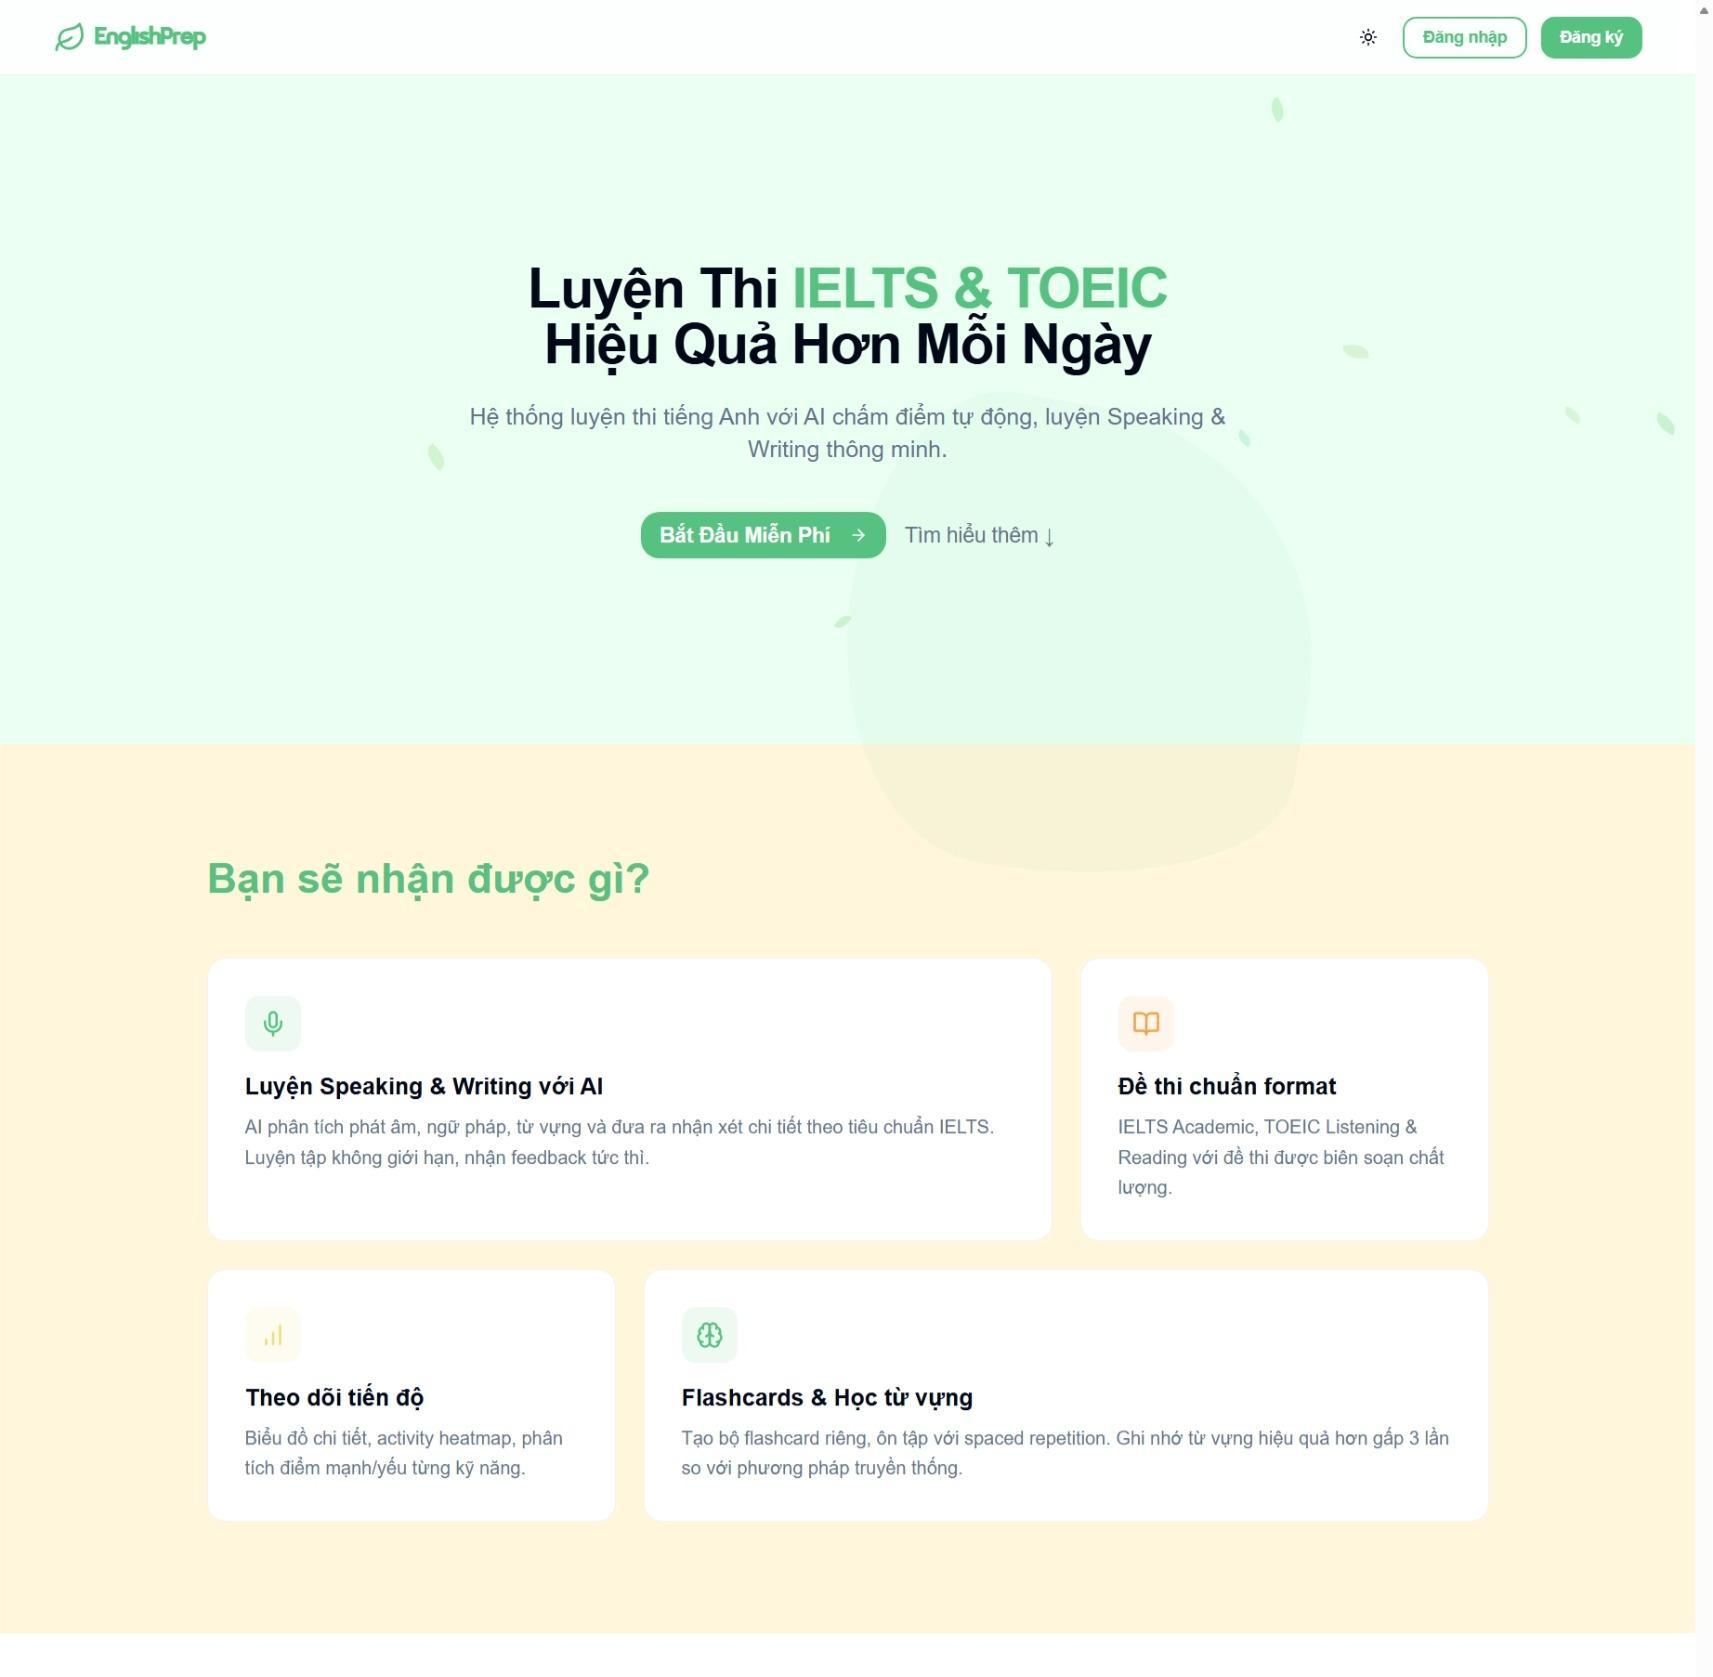
\includegraphics[width=\linewidth]{graphics/ui/homepage.jpg}
    \captionsetup{skip=5pt}
    \caption{Giao diện trang chủ}
\end{figure}
\noindent Trang chủ đóng vai trò là điểm tiếp xúc đầu tiên giữa người dùng và nền tảng. Bố cục của trang được thiết kế theo hướng tạo ấn tượng chuyên nghiệp, tăng độ tin cậy thông qua các số liệu nổi bật, mô tả ngắn gọn về công nghệ chấm điểm tự động và cơ chế học thích ứng bằng AI. Trong vùng hero, các nút hành động như ``Start for free'' và ``Watch demo'' được đặt ở vị trí nổi bật để khuyến khích người dùng nhanh chóng trải nghiệm hệ thống hoặc tìm hiểu thêm về sản phẩm. Tổng thể giao diện sử dụng phong cách tối giản, rõ ràng, giúp dẫn dắt người học từ giai đoạn quan tâm ban đầu đến bước đăng ký tài khoản một cách tự nhiên.

\subsection{Authentication Page}

\begin{figure}[H]
    \centering
    
\includegraphics[width=\linewidth]{graphics/ui/auth.jpg}
    \captionsetup{skip=5pt}
    \caption{Trang xác thực người dùng}
    \label{h8}
\end{figure}
\noindent Trang đăng nhập được thiết kế theo định hướng tập trung và tối giản nhằm giúp người dùng hoàn thành thao tác xác thực một cách nhanh chóng. Giao diện hỗ trợ nhiều phương thức đăng nhập, bao gồm tài khoản email/mật khẩu truyền thống và các lựa chọn đăng nhập qua mạng xã hội như Google hoặc Facebook. Toàn bộ nội dung chính được gom trong một thẻ trung tâm để giảm nhiễu thị giác, từ đó làm nổi bật luồng truy cập vào hệ thống học tập. Bên cạnh đó, các liên kết đăng ký tài khoản mới cũng được thể hiện rõ ràng nhằm phục vụ đồng thời cả người dùng quay lại lẫn người dùng lần đầu truy cập.

\subsection{Dashboard}

\begin{figure}[H]
    \centering
    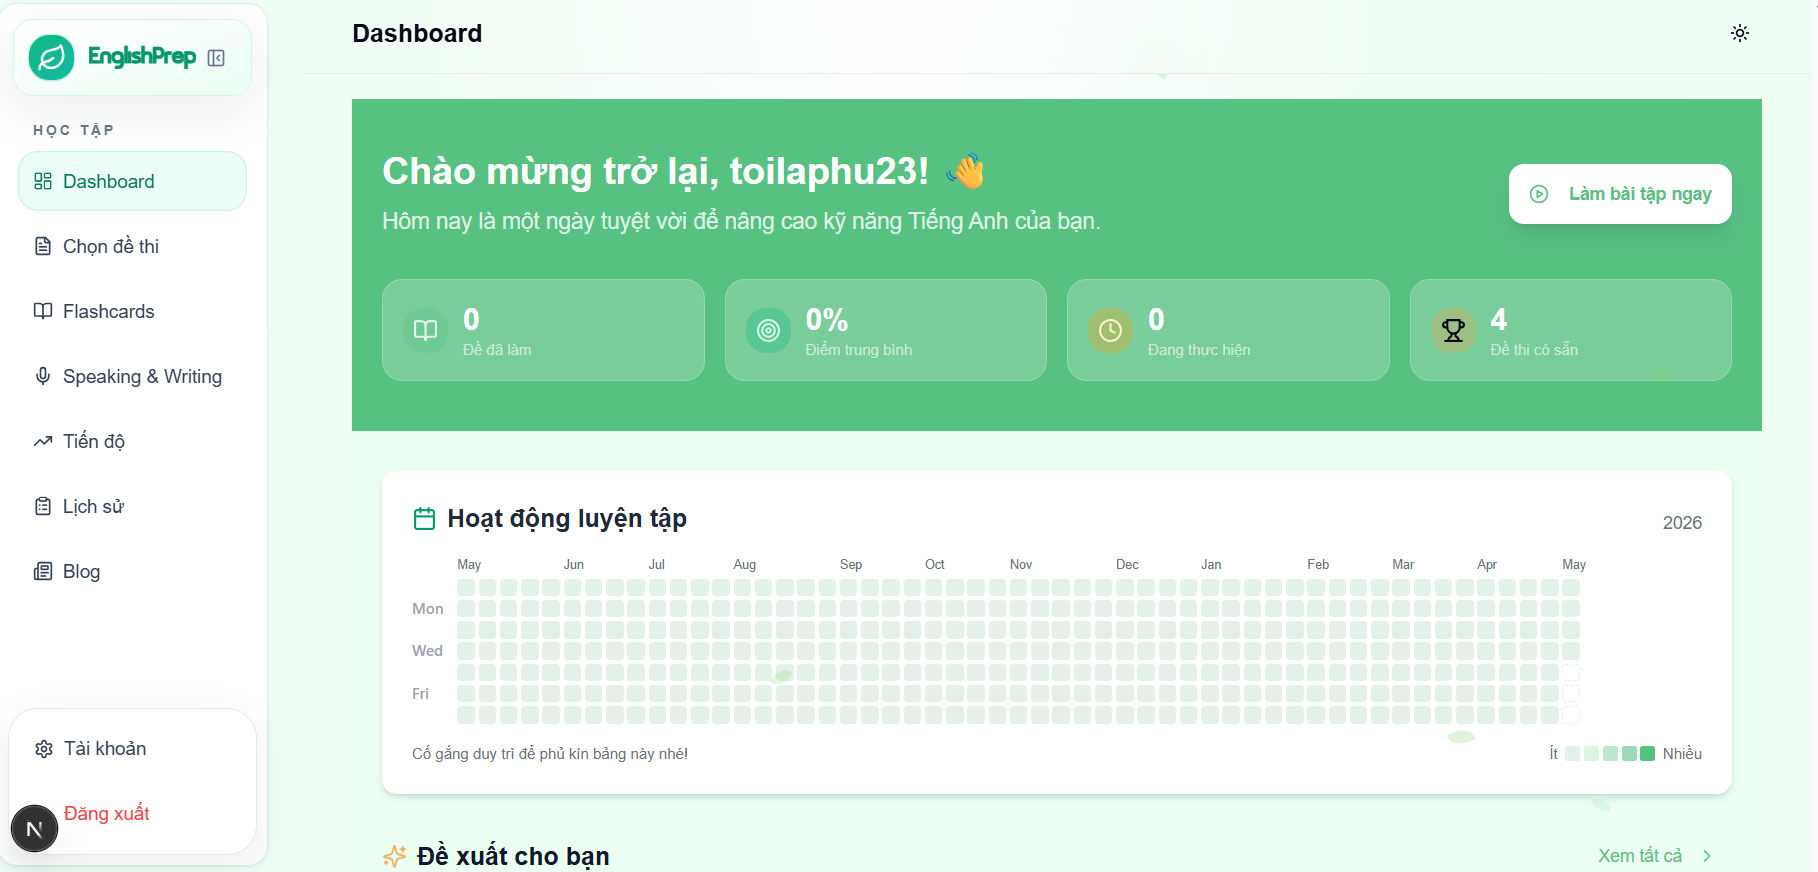
\includegraphics[width=\linewidth]{graphics/ui/dashboard.jpg}
    \captionsetup{skip=5pt}
    \caption{Bảng điều khiển người dùng}
    \label{h9}
\end{figure}
\noindent Dashboard là màn hình tổng quan đầu tiên sau khi đăng nhập, tập trung vào việc tóm tắt nhanh trạng thái học tập hiện tại của người dùng. Phần banner chào mừng ở phía trên kết hợp với nút hành động ``Làm bài tập ngay'' giúp người học bắt đầu phiên luyện tập mới một cách trực tiếp. Ngay bên dưới, các thẻ thống kê thể hiện số bài đã làm, điểm trung bình, số bài đang thực hiện và số đề thi hiện có, qua đó cung cấp một bức tranh ngắn gọn về tiến độ cá nhân. Khu vực ``Hoạt động luyện tập'' sử dụng biểu đồ nhiệt theo ngày để phản ánh mức độ duy trì thói quen học, đồng thời tạo nền tảng cho các gợi ý luyện tập tiếp theo ở phần dưới trang.

\subsection{Exam}


\begin{figure}[H]
    \centering
    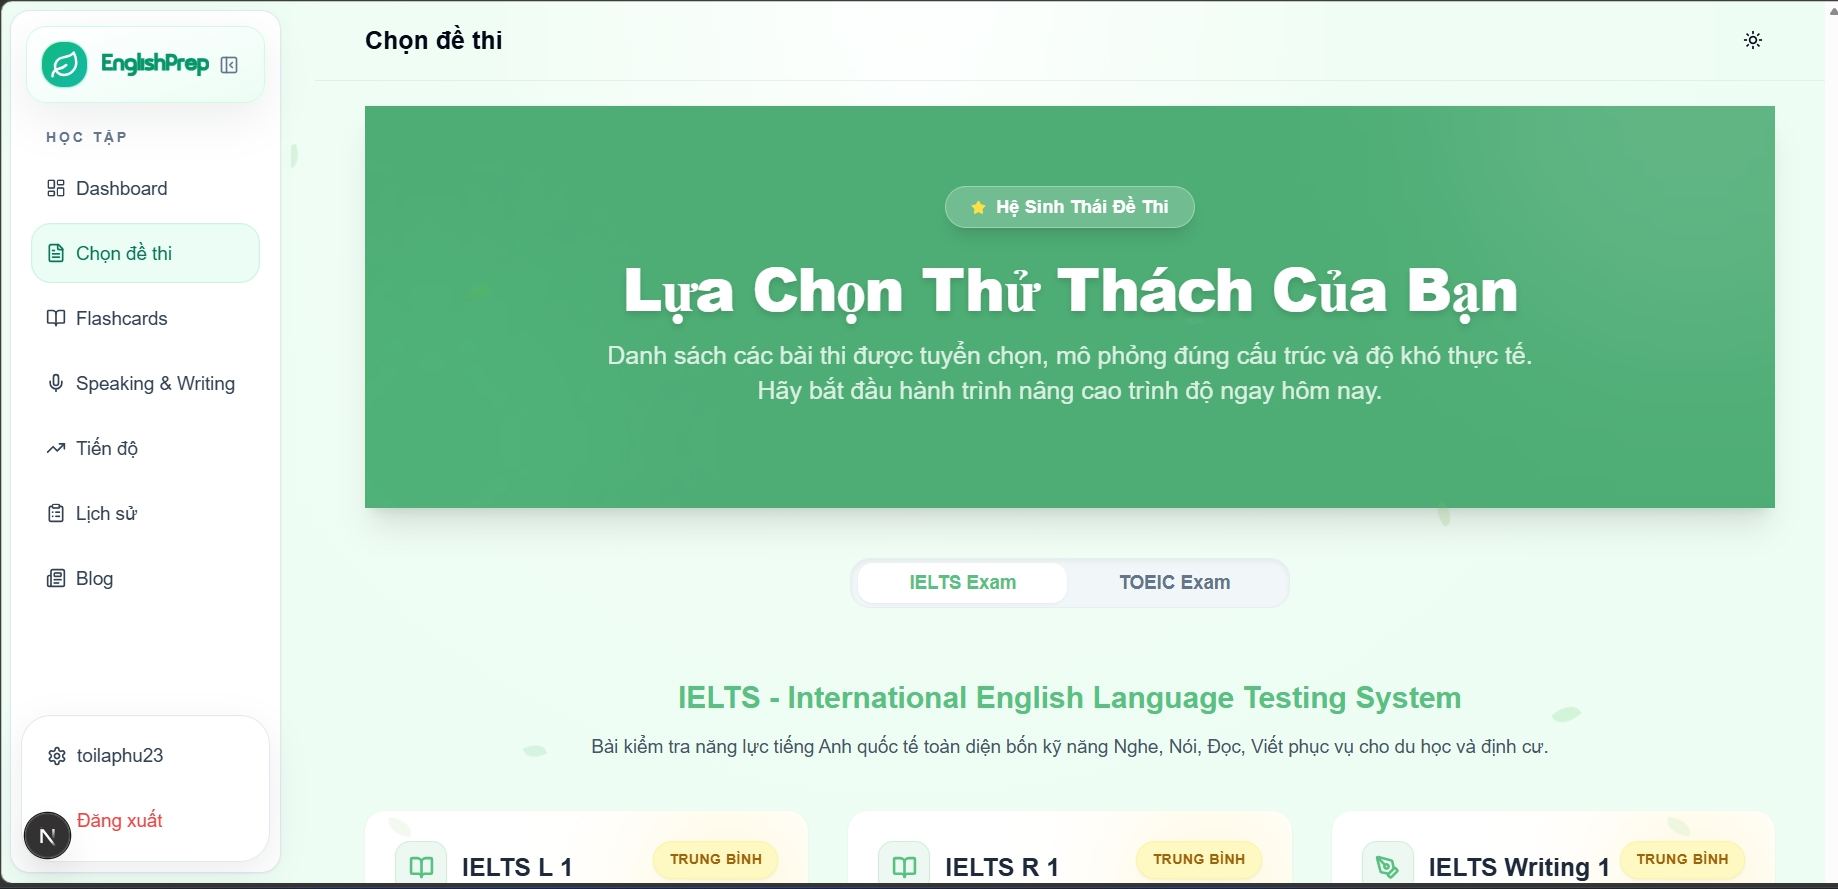
\includegraphics[width=\linewidth]{graphics/ui/exam/exam-selection.jpg}
    \captionsetup{skip=5pt}
    \caption{Giao diện lựa chọn bài thi}
    \label{h10}
\end{figure}

\noindent Trang lựa chọn bài thi cung cấp cái nhìn có hệ thống về toàn bộ tài liệu luyện tập hiện có trên nền tảng. Các đề thi được nhóm theo danh mục rõ ràng, đồng thời mỗi thẻ bài thi hiển thị những thông tin quan trọng như độ khó, thời lượng và hình thức luyện tập. Nhờ đó, người học có thể nhanh chóng so sánh, lựa chọn các đề thi mô phỏng hoặc các bài luyện chuyên sâu phù hợp với trình độ và mục tiêu của mình.

\begin{figure}[H]
    \centering
    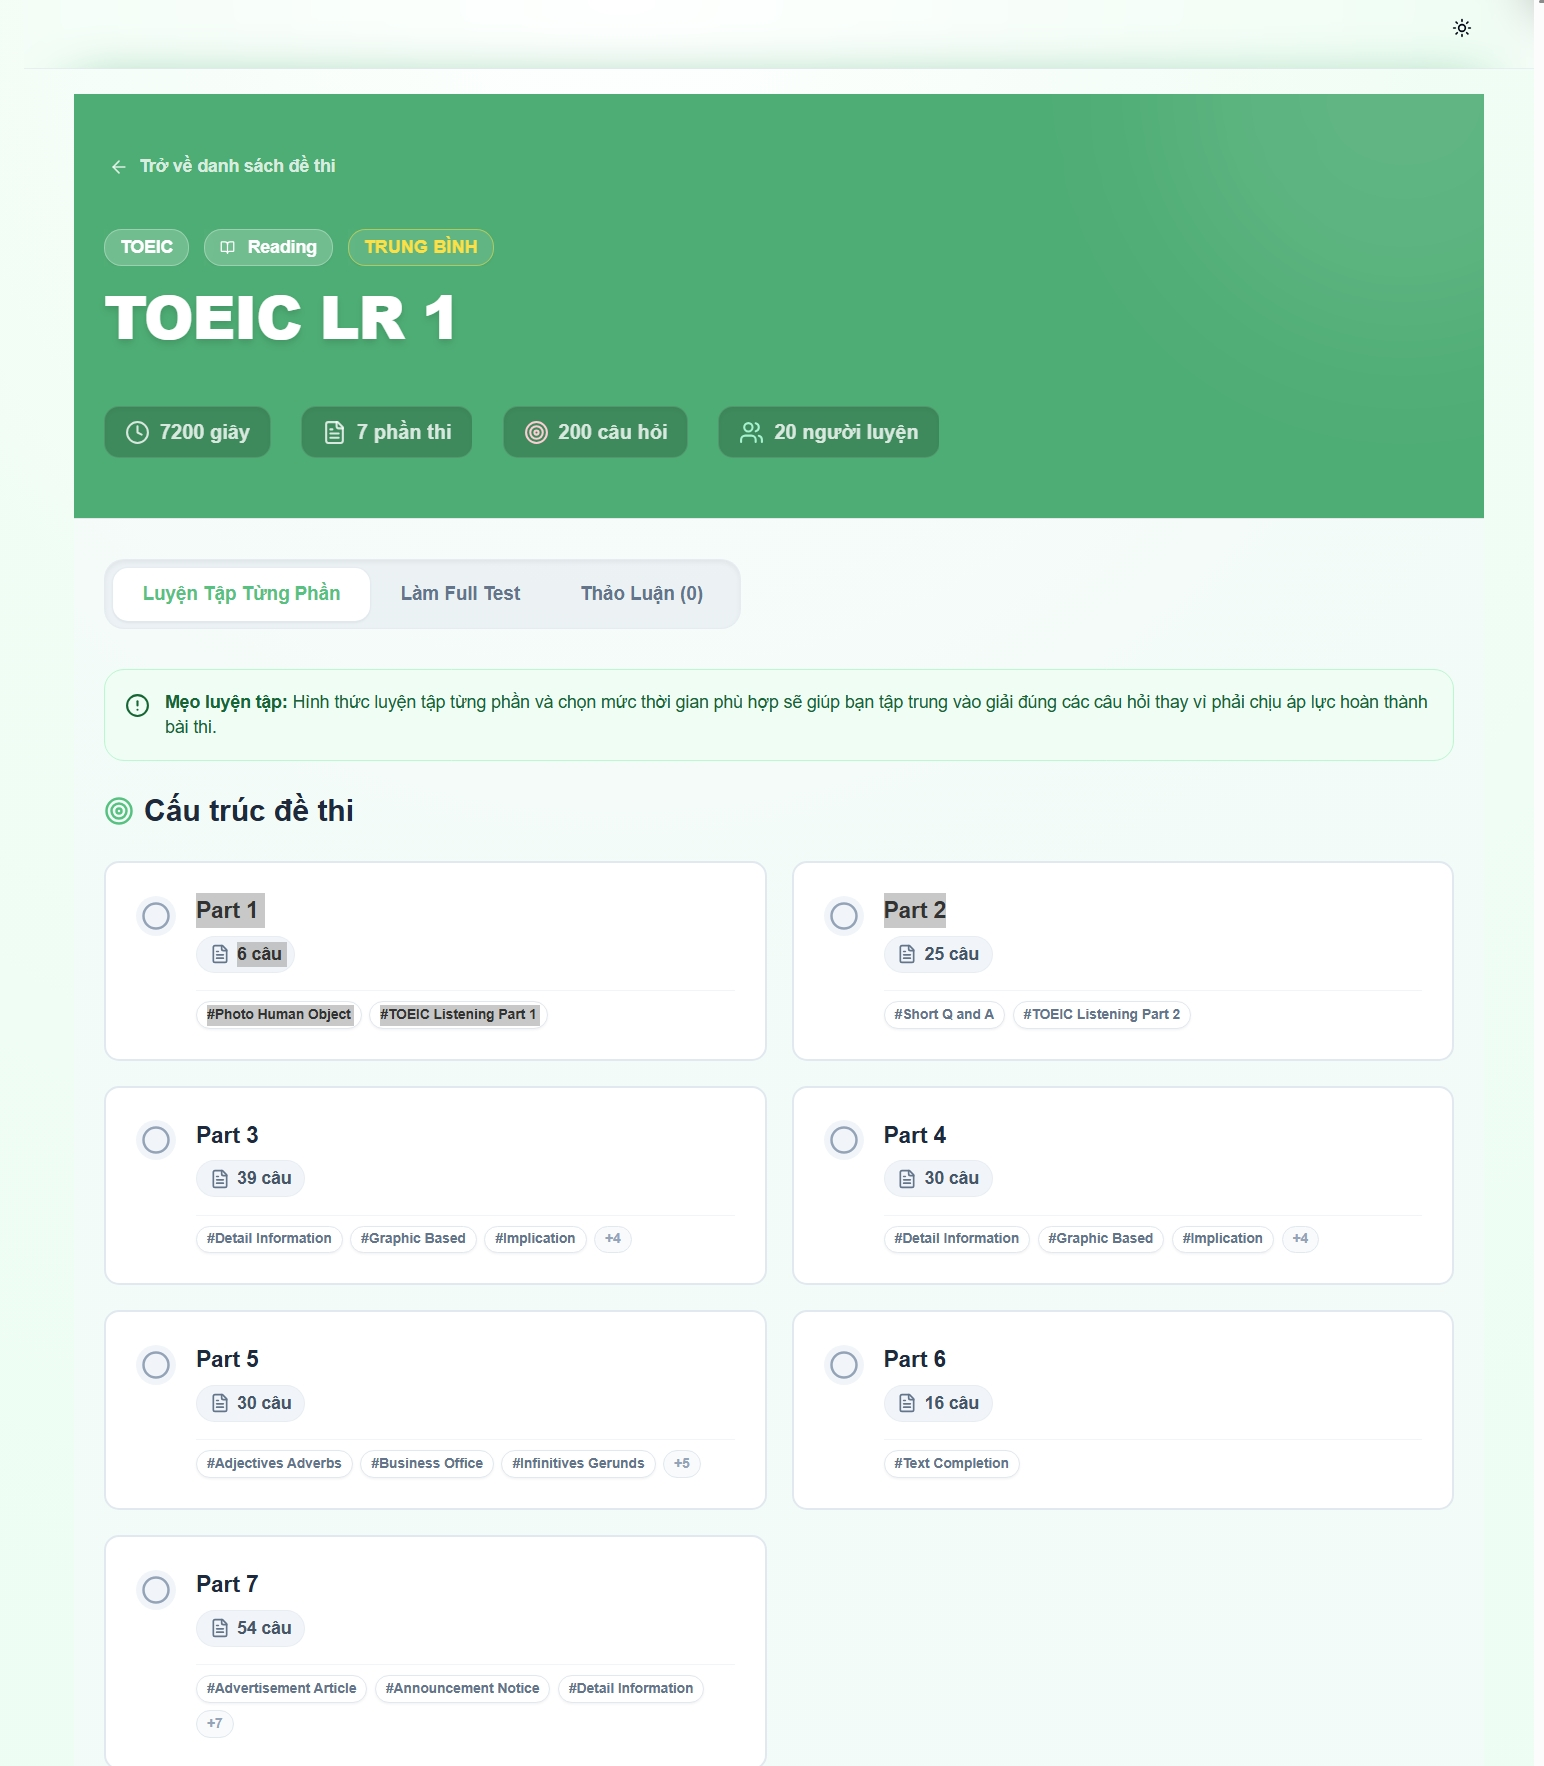
\includegraphics[width=\linewidth]{graphics/ui/exam/exam-detail.jpg}
    \captionsetup{skip=5pt}
    \caption{Giao diện chi tiết bài thi}
    \label{h11}
\end{figure}
\noindent Trang chi tiết bài thi trình bày đầy đủ thông tin và các tùy chọn cấu hình trước khi người dùng bắt đầu làm bài. Bố cục sạch và rõ ràng giúp làm nổi bật các thông số như thời lượng, số lượng câu hỏi và mức độ khó, đồng thời cho phép lựa chọn chế độ làm bài có bấm giờ hoặc không bấm giờ. Người dùng có thể bắt đầu toàn bộ đề thi ngay lập tức hoặc chọn từng phần cụ thể để luyện tập theo nhu cầu. Bên cạnh đó, khu vực thảo luận và đánh giá còn hỗ trợ người học tham khảo nhận xét từ cộng đồng để hình dung trước chất lượng và độ thử thách của bài thi.

\begin{figure}[H]
    \centering
    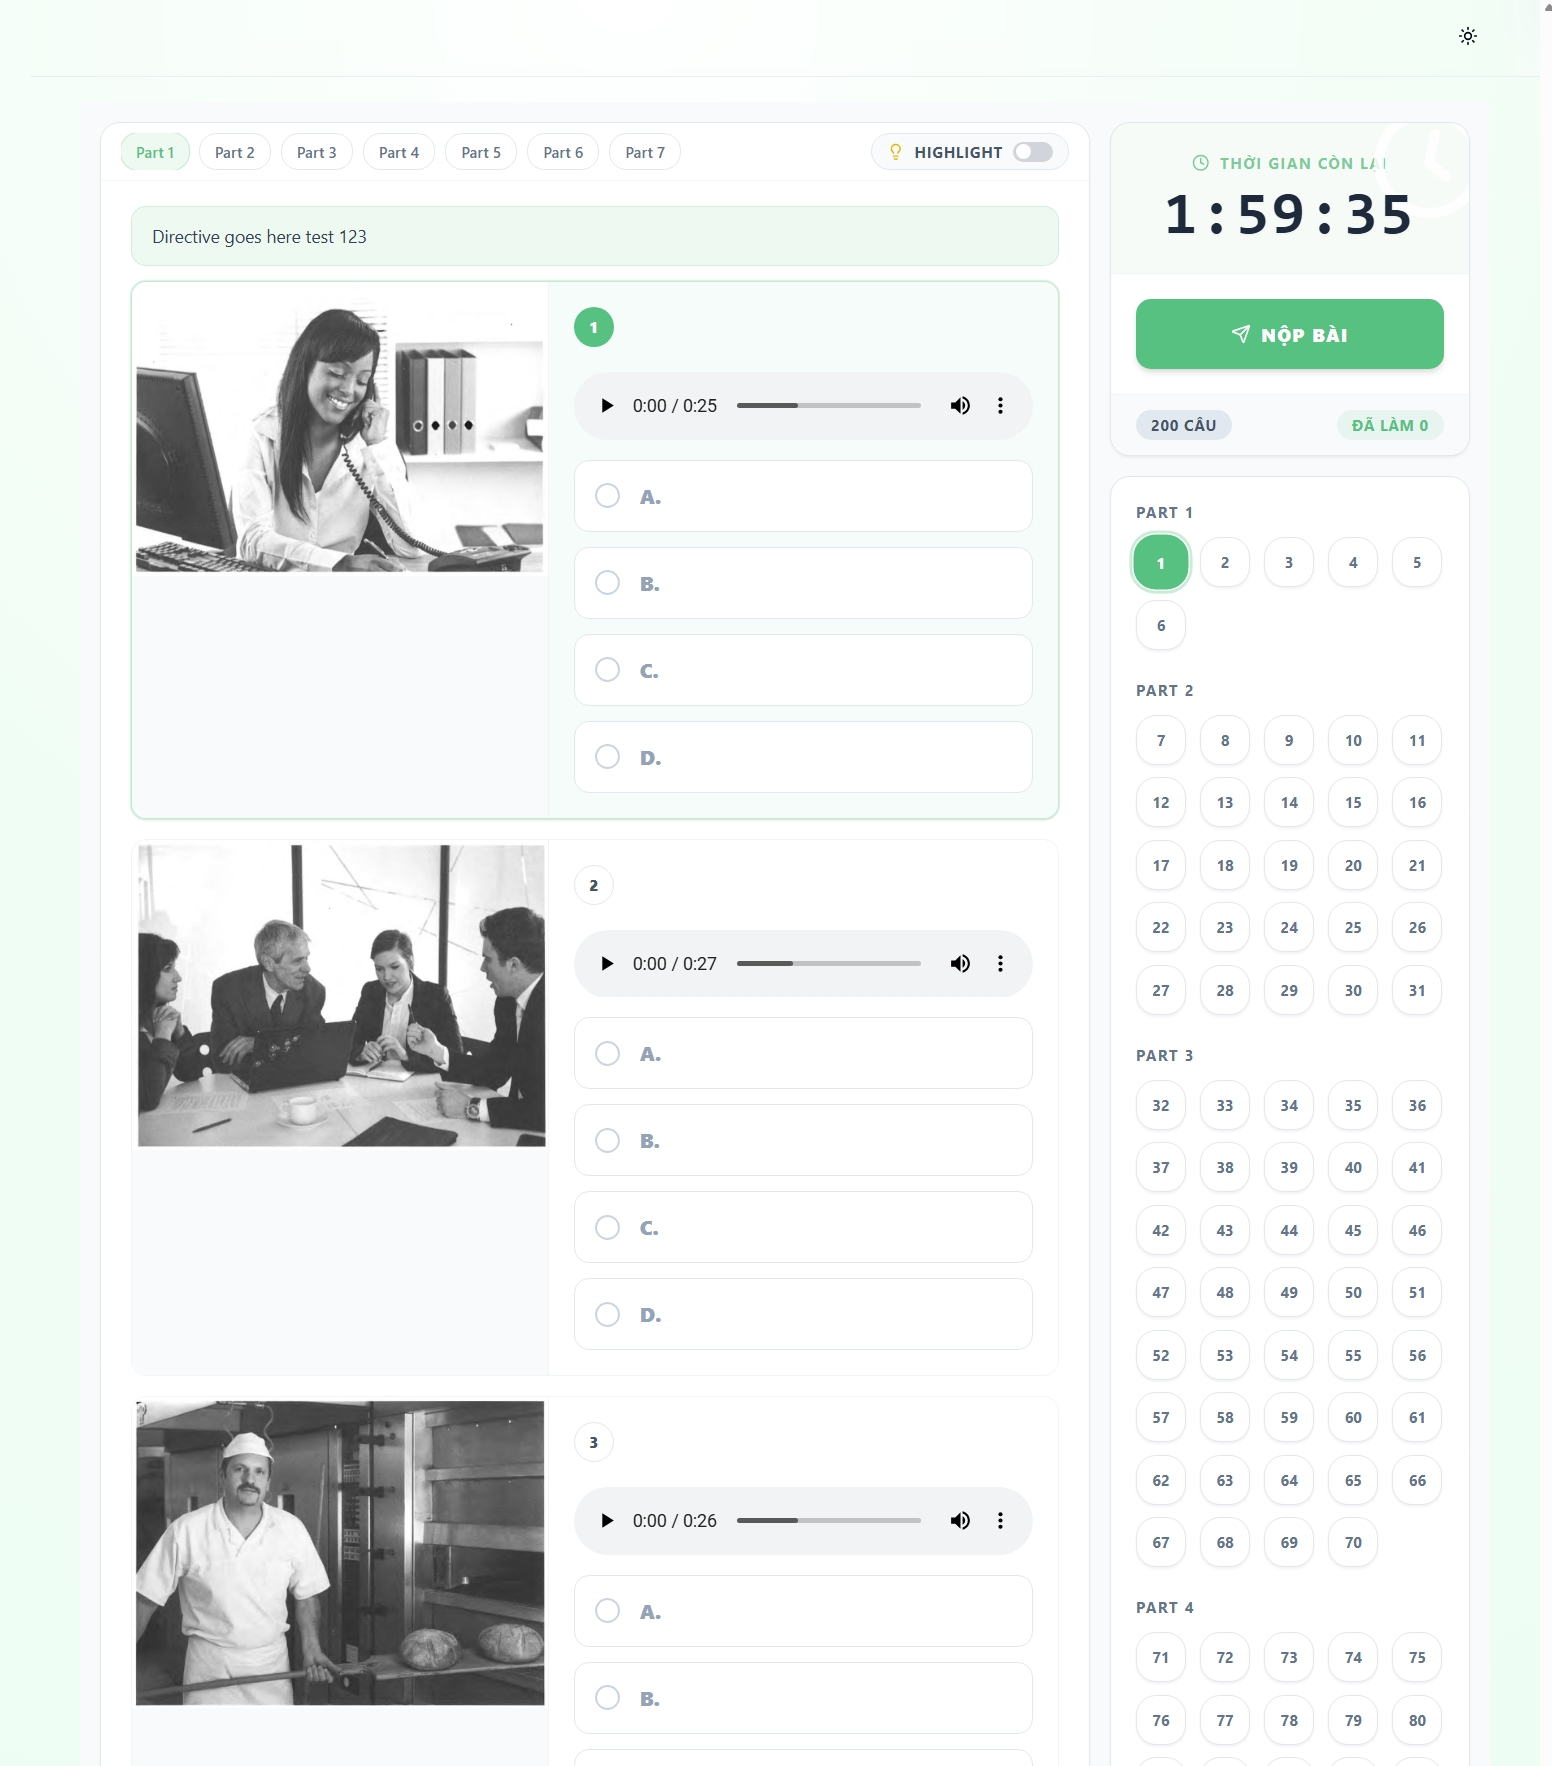
\includegraphics[width=\linewidth]{graphics/ui/exam/exam-interface.jpg}
    \captionsetup{skip=5pt}
    \caption{Giao diện làm bài thi}
    \label{h12}
\end{figure}
\noindent Giao diện làm bài được thiết kế nhằm tạo ra môi trường tập trung và sát với trải nghiệm thi thật. Bố cục chia tách hợp lý giữa phần nội dung đọc và khu vực trả lời giúp người dùng vừa theo dõi đề bài vừa thao tác trả lời một cách thuận tiện. Các công cụ phụ trợ như bộ đếm thời gian và trình điều hướng câu hỏi hỗ trợ người học kiểm soát chiến lược làm bài hiệu quả hơn. Trong trường hợp muốn kết thúc sớm, người dùng có thể chủ động nộp bài thông qua nút Submit được bố trí rõ ràng.

\begin{figure}[H]
    \centering
    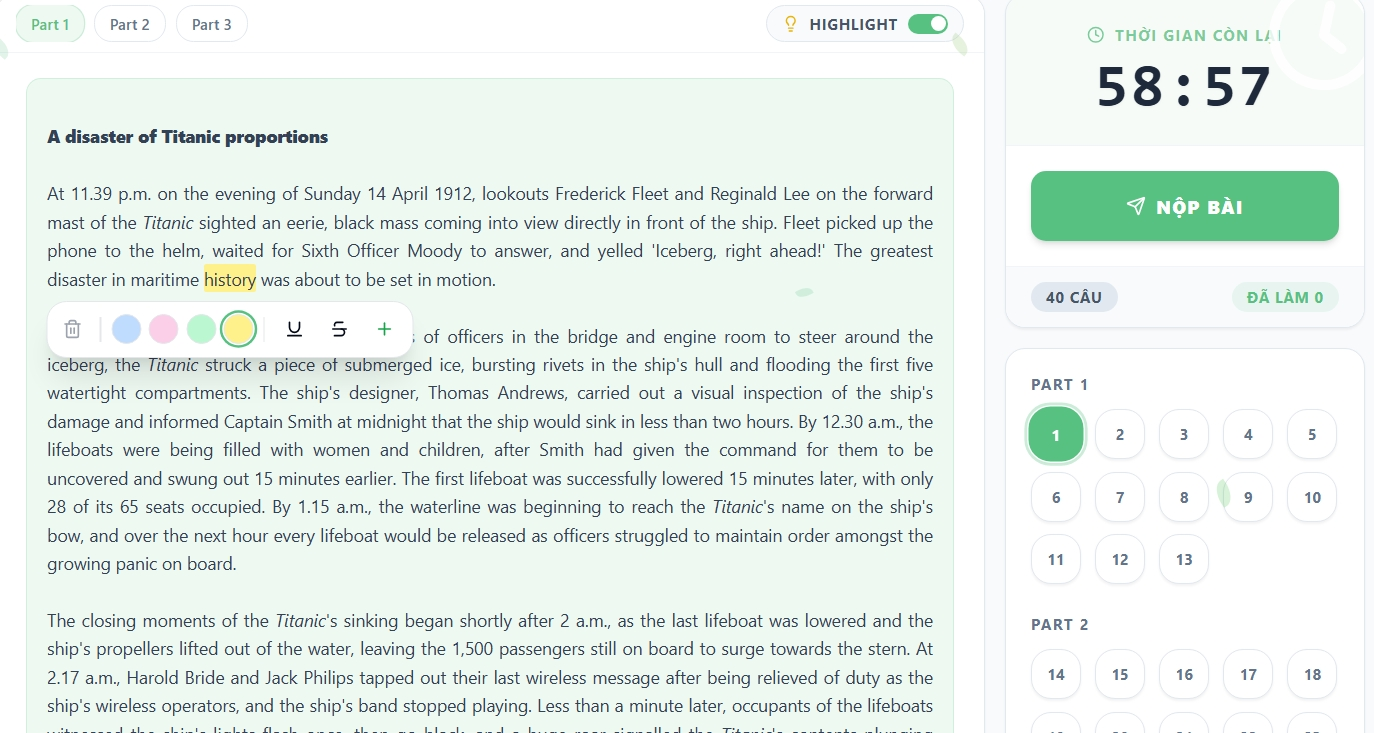
\includegraphics[width=\linewidth]{graphics/ui/exam/exam-interface-highlight.jpg}
    \captionsetup{skip=5pt}
    \caption{Công cụ tô sáng và ghi chú văn bản}
    \label{h12_highlight}
\end{figure}
\noindent Bên cạnh chức năng làm bài cơ bản, hệ thống còn cung cấp bộ công cụ chú thích số nhằm nâng cao hiệu quả đọc hiểu trong quá trình luyện tập. Người dùng có thể tô sáng nhiều màu, định dạng văn bản, tra cứu từ điển trực tuyến hoặc tạo ghi chú trực tiếp từ đoạn văn đang đọc. Những công cụ này giúp học viên nhanh chóng đánh dấu ý chính, lưu lại bằng chứng quan trọng cho câu hỏi và tổ chức thông tin một cách có hệ thống hơn.

\begin{figure}[H]
    \centering
    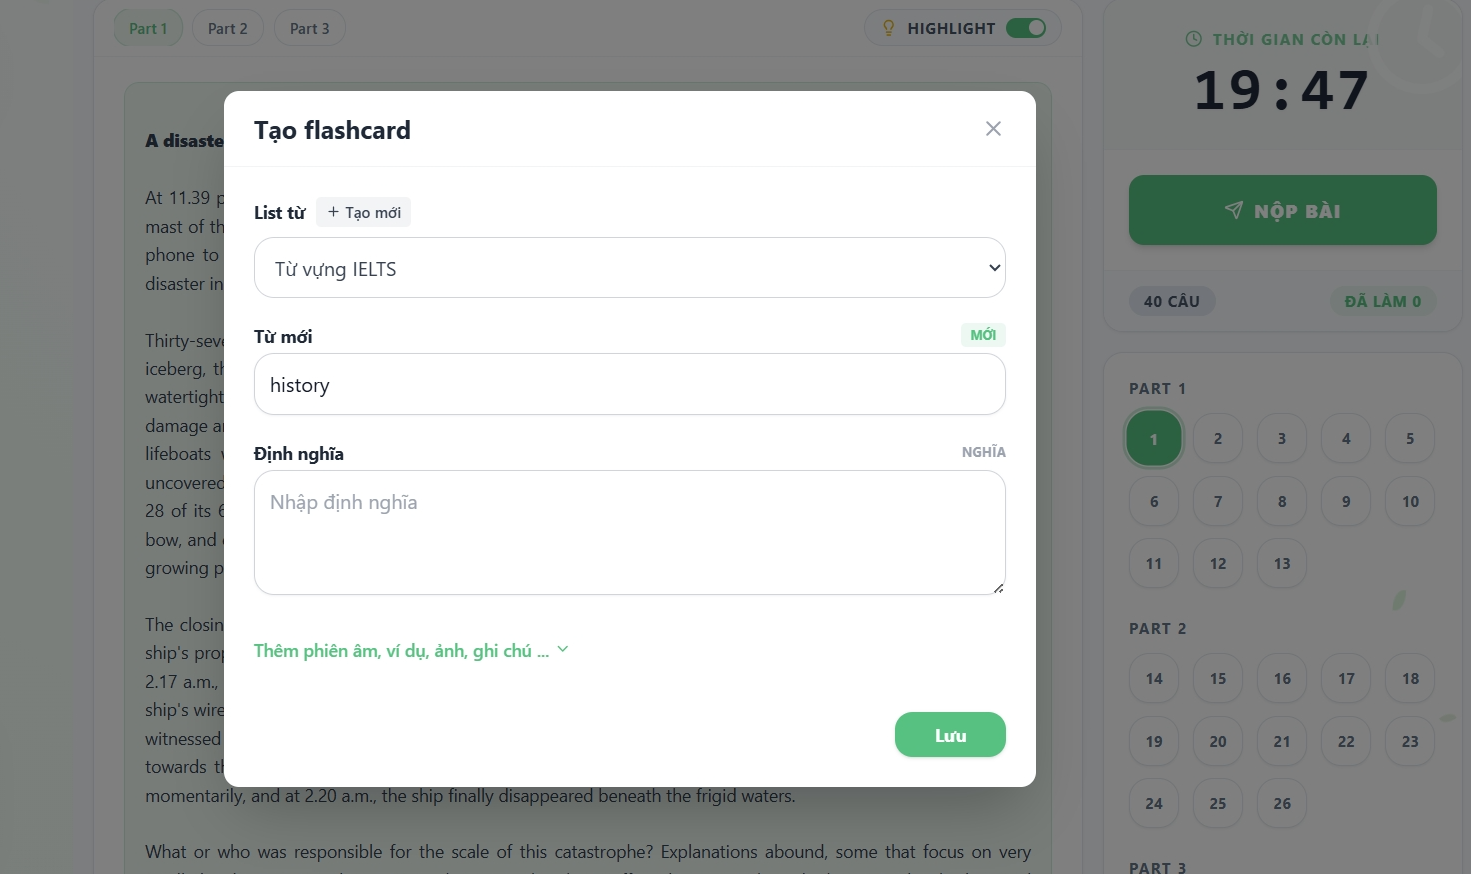
\includegraphics[width=\linewidth]{graphics/ui/exam/exam-interface-create-flashcard.jpg}
    \captionsetup{skip=5pt}
    \caption{Tạo flashcard ngay trong lúc làm bài}
    \label{h12_flashcard}
\end{figure}
\noindent Một điểm nổi bật của hệ thống là khả năng tạo flashcard trực tiếp từ nội dung được tô sáng ngay trong bài thi. Tính năng này giúp giảm khoảng cách giữa quá trình phát hiện từ vựng mới và việc lưu trữ để ôn tập về sau. Hộp thoại tạo flashcard được thiết kế đơn giản, hỗ trợ lưu nhanh hoặc bổ sung ghi chú ngôn ngữ chi tiết, từ đó biến mỗi lần luyện đề thành một cơ hội tích lũy kiến thức lâu dài và có tính cá nhân hóa cao.

\begin{figure}[H]
    \centering
    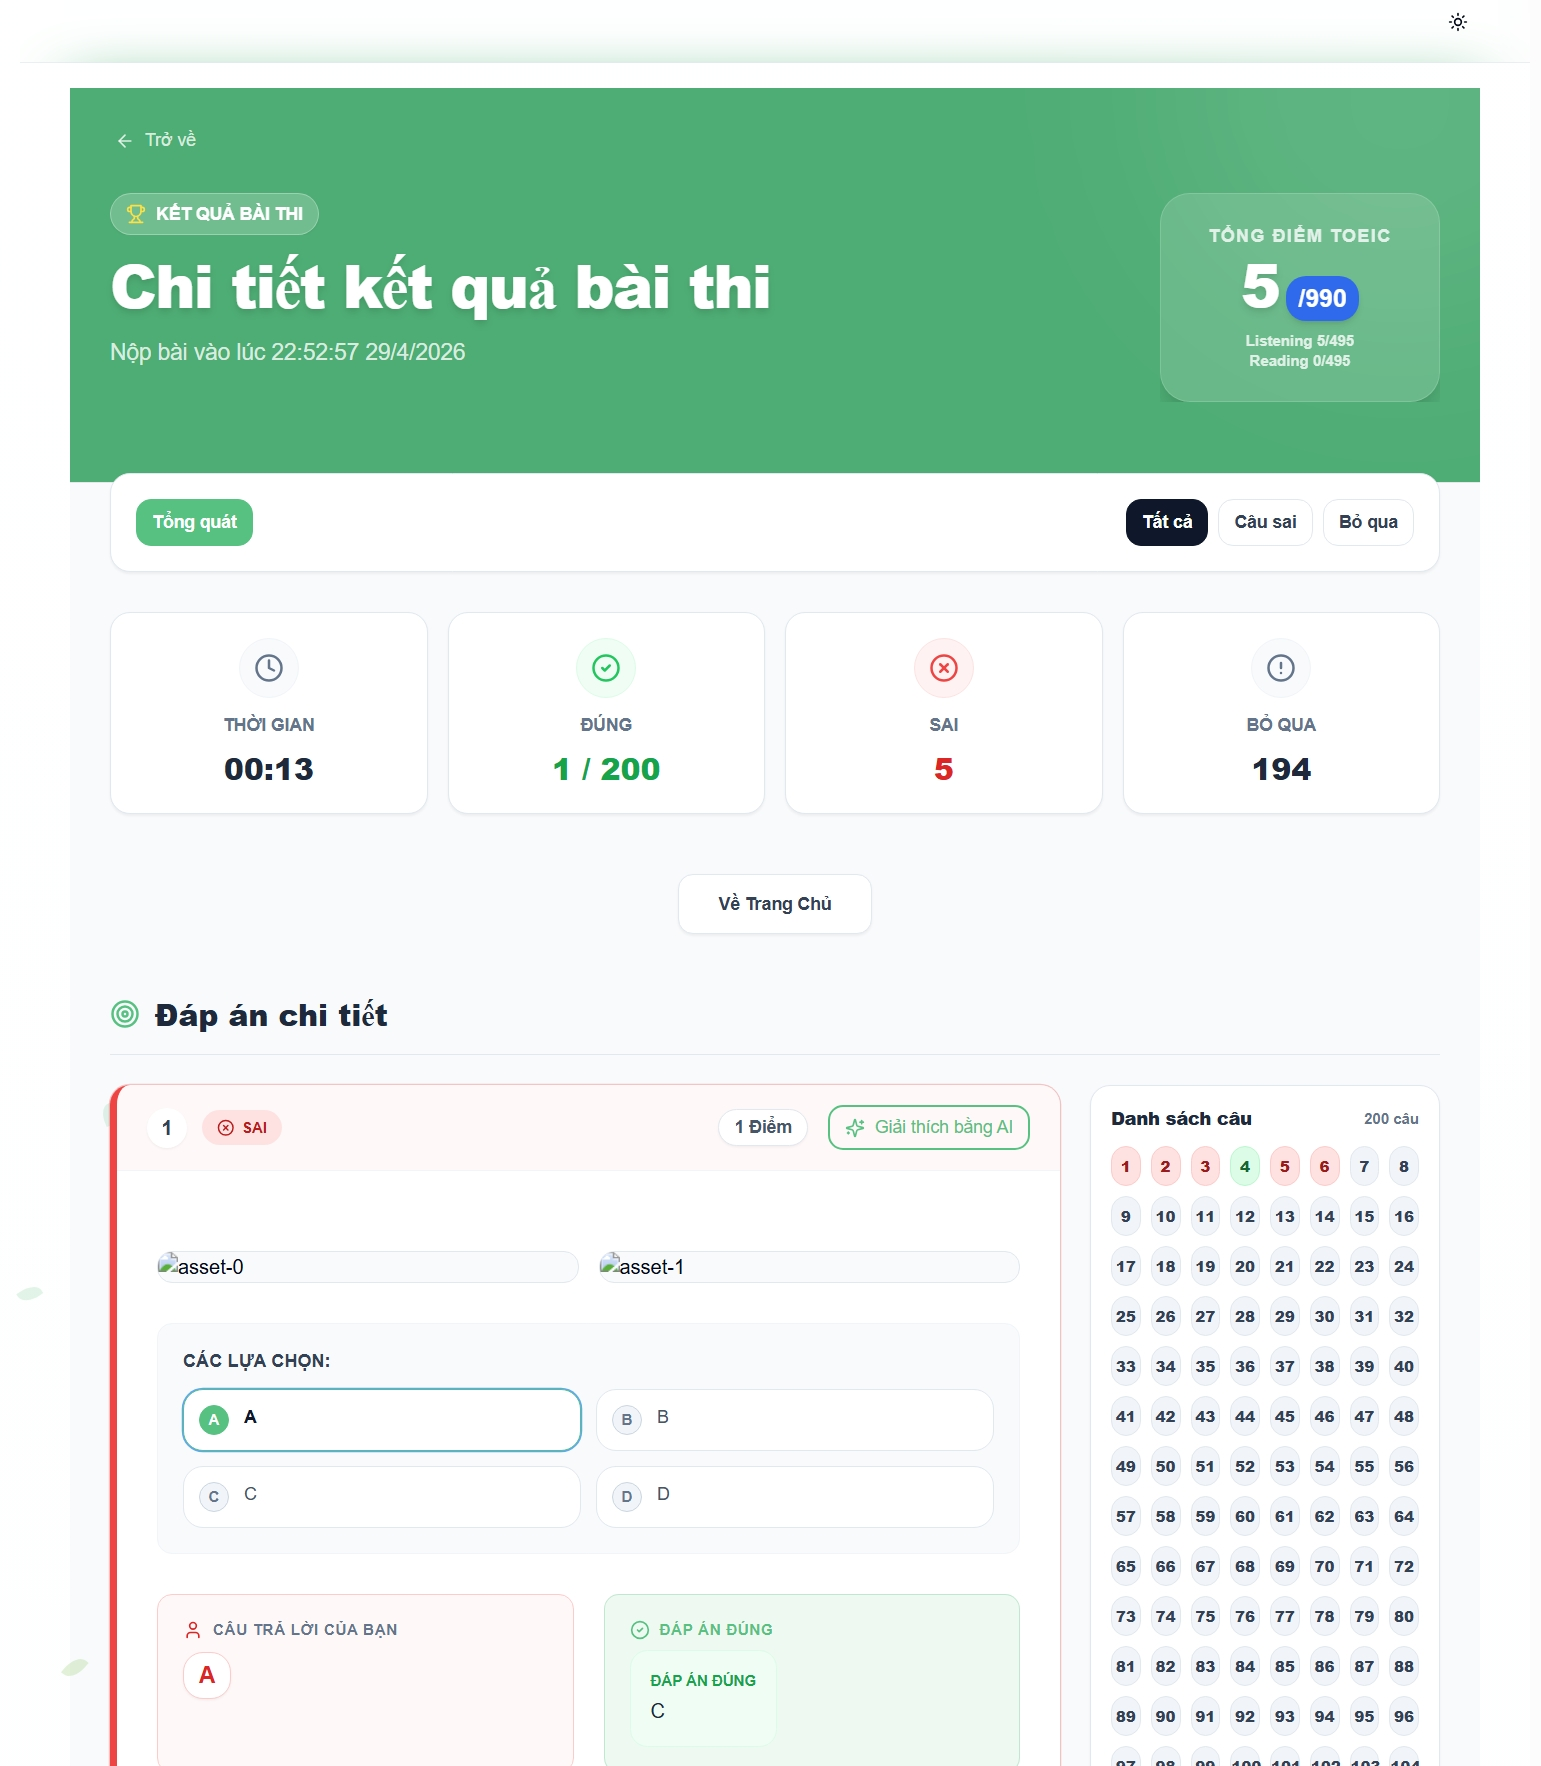
\includegraphics[width=\linewidth]{graphics/ui/exam/exam-result.jpg}
    \captionsetup{skip=5pt}
    \caption{Kết quả và phân tích bài thi}
    \label{h13}
\end{figure}
\noindent Sau khi hoàn thành bài thi, người dùng nhận được phản hồi tức thì bao gồm tổng điểm, thời gian hoàn thành và bảng phân tích chi tiết các câu đúng, sai để phục vụ cho việc rà soát. Cách trình bày kết quả theo hướng trực quan giúp người học dễ dàng nhận biết mức độ hoàn thành bài làm cũng như xác định các phần kiến thức cần cải thiện.


\subsection{Speaking Test}

\begin{figure}[H]
    \centering
    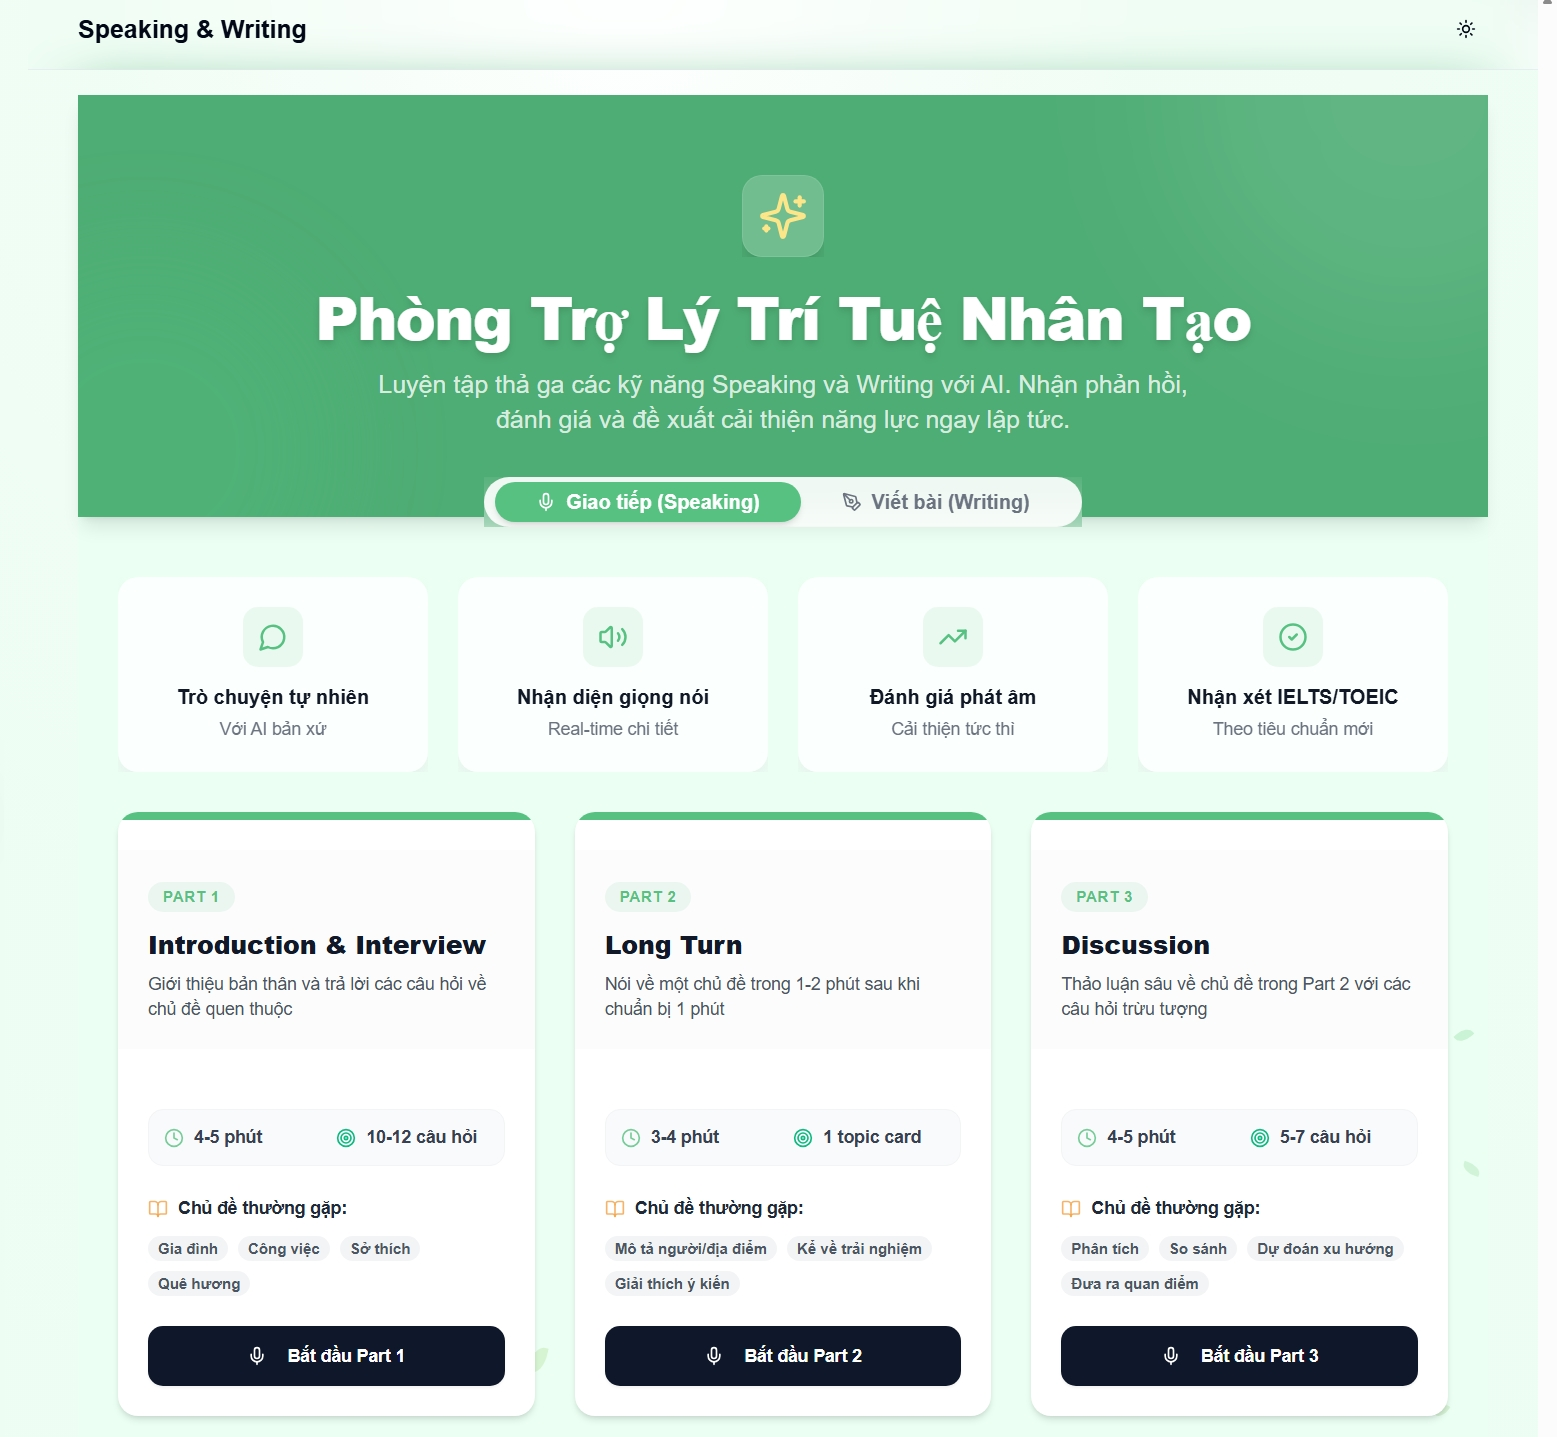
\includegraphics[width=\linewidth]{graphics/ui/exam/speaking-selection.jpg}
    \captionsetup{skip=5pt}
    \caption{Tổng quan và lựa chọn bài thi nói}
\end{figure}
\noindent Giao diện tổng quan bài thi Speaking đóng vai trò như cổng truy cập cho chức năng luyện nói với AI. Các phần luyện tập được chia theo cấu trúc logic của bài thi, giúp người dùng dễ dàng lựa chọn đúng dạng câu hỏi hoặc chủ đề cần rèn luyện. Bố cục đồng thời nhấn mạnh các năng lực nổi bật của hệ thống như ghi âm, chuyển giọng nói thành văn bản theo thời gian thực và cơ chế đặt câu hỏi thích ứng, từ đó tạo tiền đề cho một buổi luyện nói hiệu quả.

\begin{figure}[H]
    \centering
    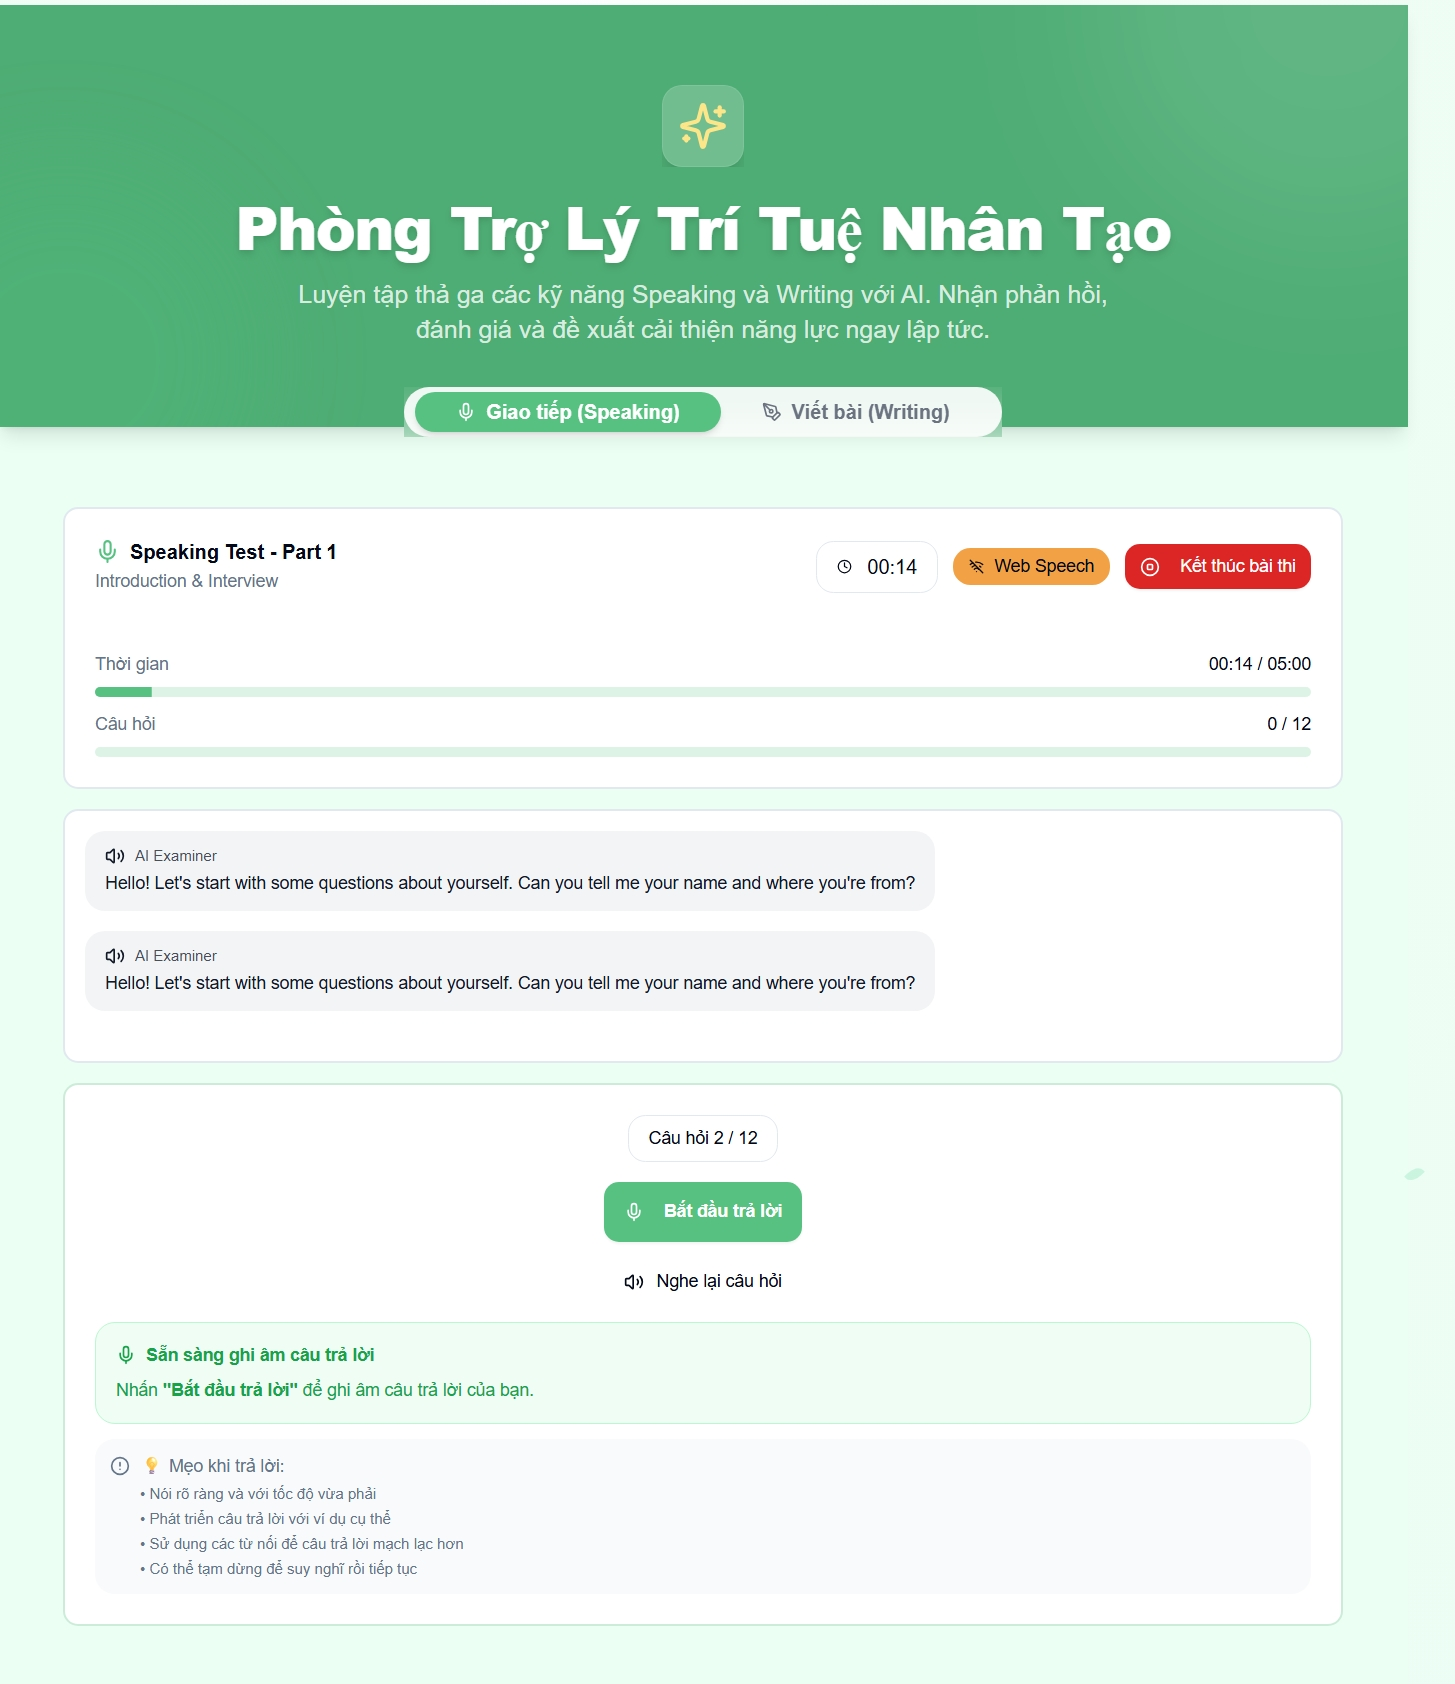
\includegraphics[width=\linewidth]{graphics/ui/exam/speaking-test-interface-during-speak.jpg}
    \captionsetup{skip=5pt}
    \caption{Giai đoạn ghi âm trực tiếp}
\end{figure}
\noindent Khi bước vào phần trả lời, giao diện tập trung vào việc hỗ trợ quá trình chuyển từ nghe hiểu sang phát biểu chủ động. Công nghệ nhận diện giọng nói theo thời gian thực cung cấp tín hiệu trực quan để người dùng biết rằng câu trả lời đang được ghi nhận chính xác. Các thành phần như đồng hồ ghi âm, trạng thái hệ thống và nút ``Finish answer'' được đặt ở vị trí dễ theo dõi nhằm giúp người học tập trung tối đa vào nội dung nói. Nhờ môi trường phản hồi nhanh và có cấu trúc, nền tảng hỗ trợ người học phát triển độ trôi chảy và sự tự tin cần thiết cho các bài thi nói thực tế.

\begin{figure}[H]
    \centering
    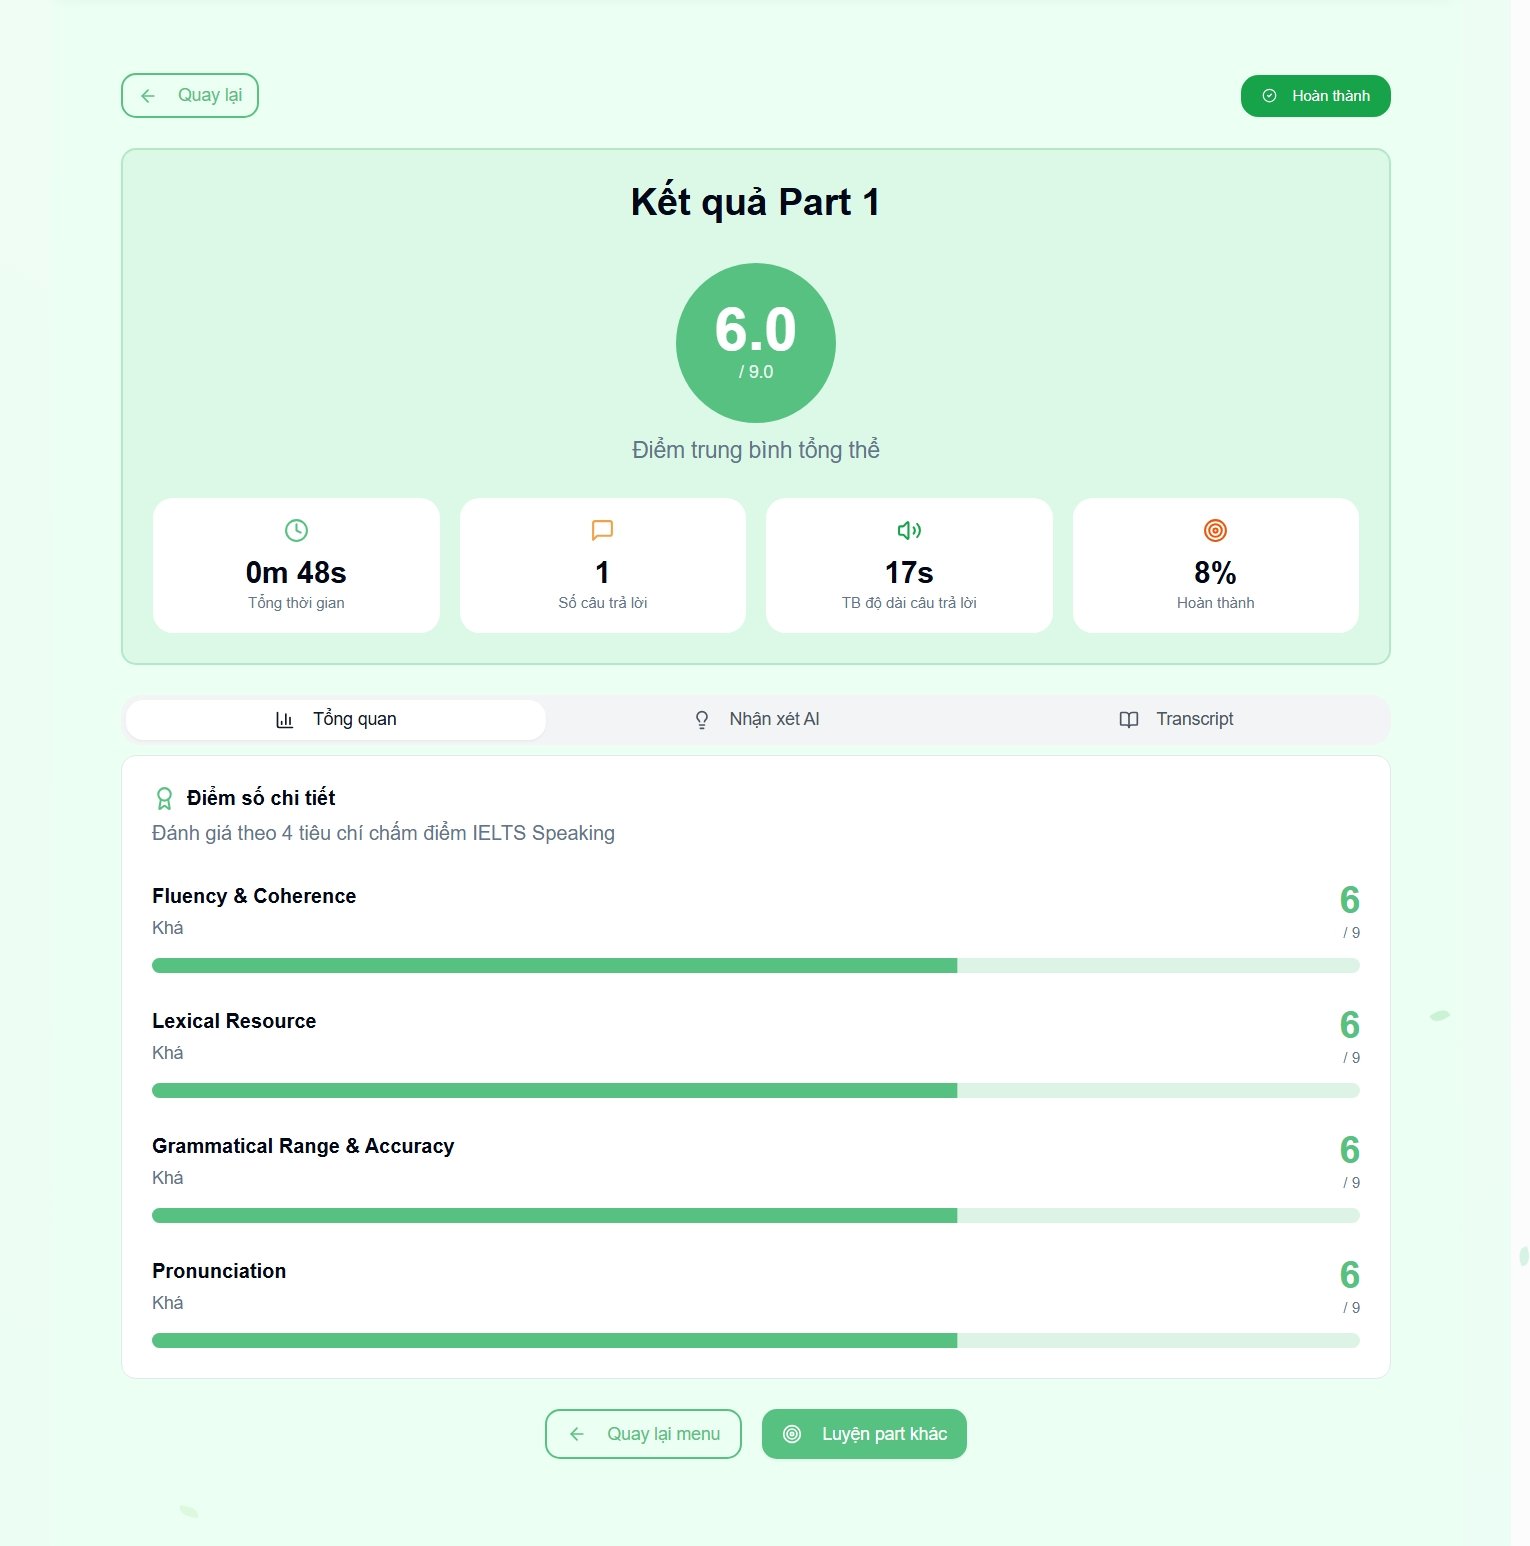
\includegraphics[width=\linewidth]{graphics/ui/exam/speaking-result.jpg}
    \captionsetup{skip=5pt}
    \caption{Kết quả bài thi nói}
\end{figure}
\noindent Sau khi kết thúc phần trả lời, hệ thống hiển thị trang kết quả Speaking với cách trình bày tập trung vào khả năng tự đánh giá và cải thiện. Vùng thông tin đầu trang cho biết điểm trung bình, tổng thời gian trả lời, số câu đã hoàn thành và thời lượng trung bình cho mỗi câu. Bên dưới, các thẻ điều hướng cho phép chuyển giữa phần tổng quan, nhận xét AI và bản transcript, giúp người dùng xem lại bài nói dưới nhiều góc độ. Phần chấm điểm chi tiết theo các tiêu chí như Fluency \& Coherence, Lexical Resource, Grammatical Range \& Accuracy và Pronunciation giúp người học hiểu rõ thành phần nào đang kéo điểm xuống để điều chỉnh chiến lược luyện nói ở các lượt sau.

\subsection{Writing Test}

\begin{figure}[H]
    \centering
    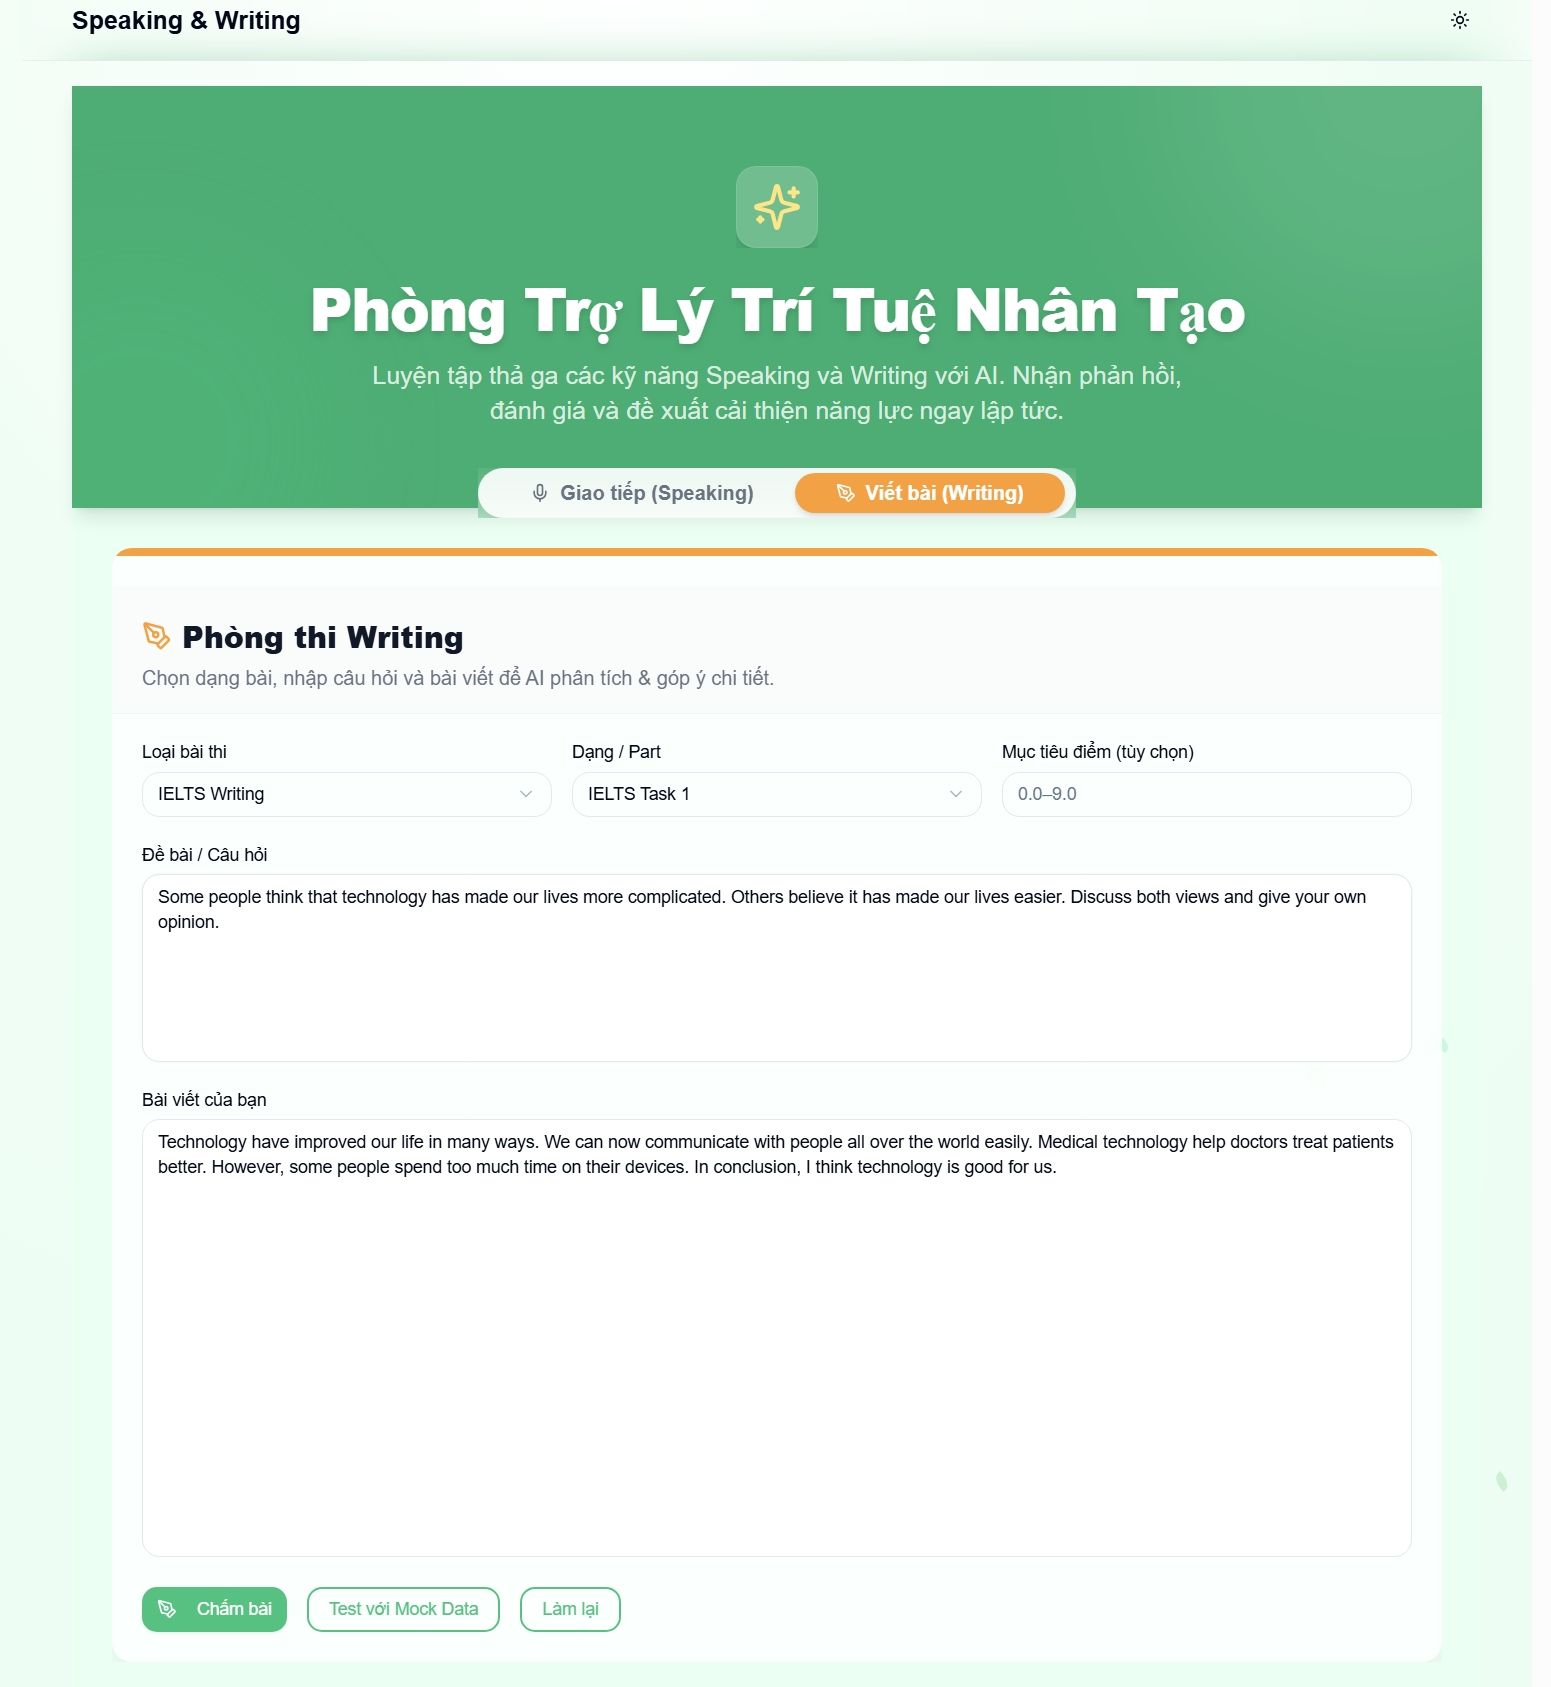
\includegraphics[width=\linewidth]{graphics/ui/exam/writing-interface.jpg}
    \captionsetup{skip=5pt}
    \caption{Giao diện bài thi viết}
    \label{fig:writing-interface}
\end{figure}
\noindent Giao diện Writing cung cấp một không gian làm việc tập trung để người học phát triển kỹ năng viết luận. Bố cục theo chiều dọc giúp người dùng lần lượt thiết lập thông số bài thi, đọc đề bài theo phong cách đề thật và nhập bài viết trong một vùng soạn thảo rõ ràng. Nút ``Grade'' được bố trí nổi bật nhằm rút ngắn quá trình chuyển từ viết sang nhận phản hồi chấm điểm bằng AI, qua đó tăng tính liên tục trong trải nghiệm học tập.

\begin{figure}[H]
    \centering
    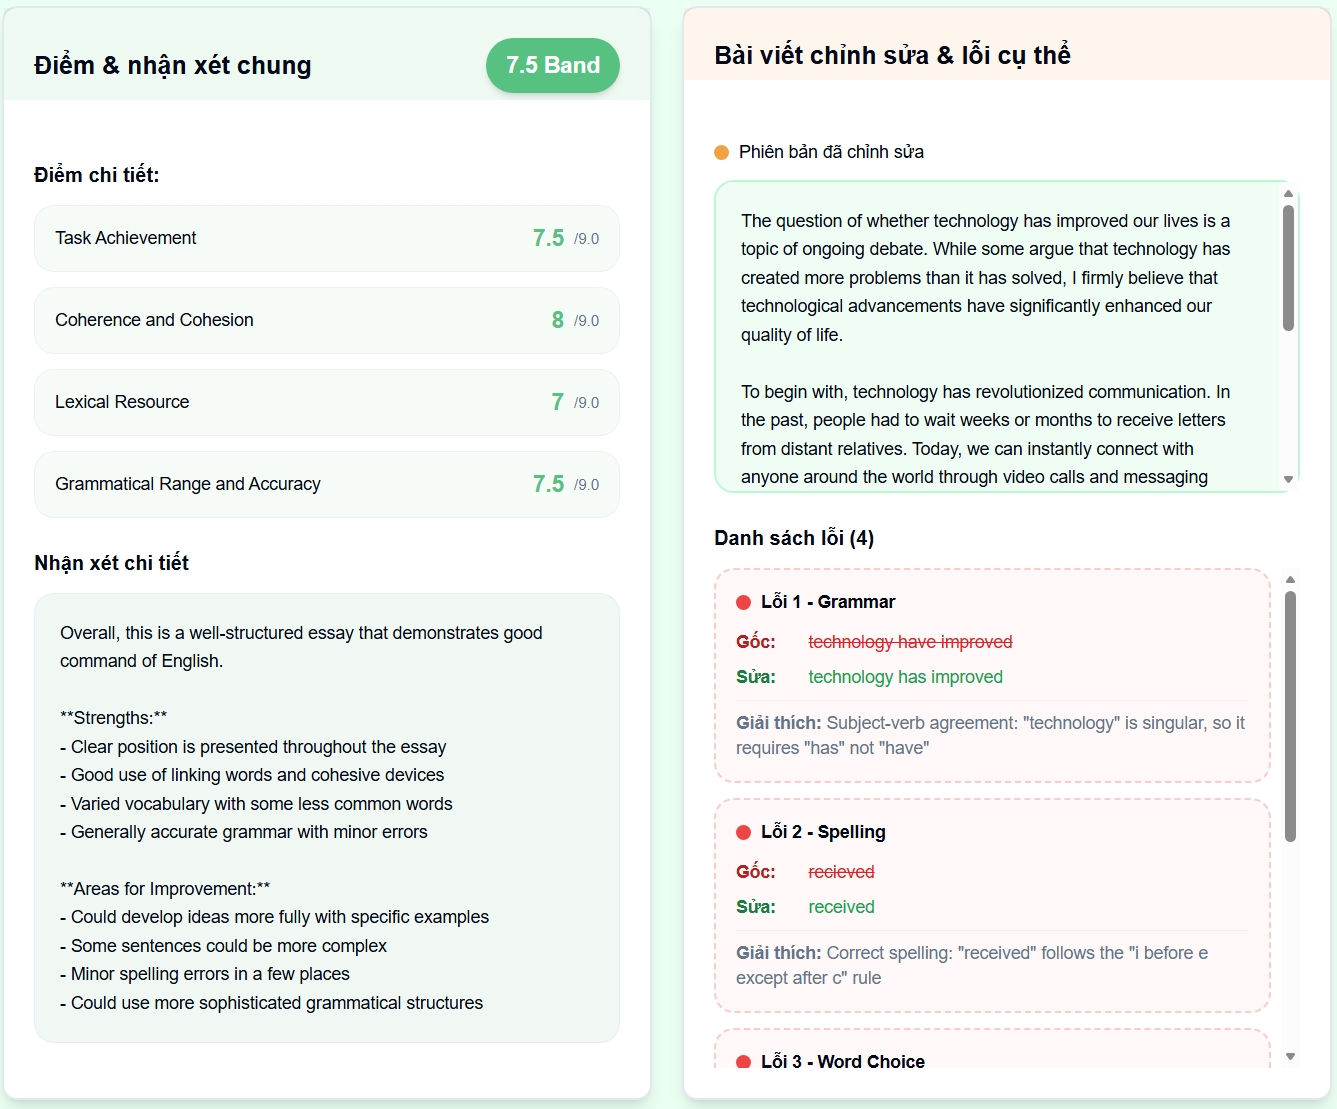
\includegraphics[width=\linewidth]{graphics/ui/exam/result-writing-interface.jpg}
    \captionsetup{skip=5pt}
    \caption{Kết quả bài thi viết}
\end{figure}

\noindent Sau khi hoàn thành bài viết, người dùng được chuyển đến trang kết quả để xem điểm số, phân tích theo từng tiêu chí và các nhận xét định tính. Trước hết, người học có thể xác định kỹ năng nào còn yếu thông qua band score và phần phân rã tiêu chí. Tiếp theo, phần nhận xét giải thích nguyên nhân của mức điểm giúp người dùng hiểu sâu hơn thay vì chỉ nhìn vào con số. Cuối cùng, khu vực so sánh câu gốc với phiên bản được AI đề xuất chỉnh sửa cho phép người học nhận diện rõ lỗi ngữ pháp, từ vựng hoặc cách diễn đạt để tránh lặp lại trong các bài viết sau.

\subsection{Flashcard}

\begin{figure}[H]
    \centering
    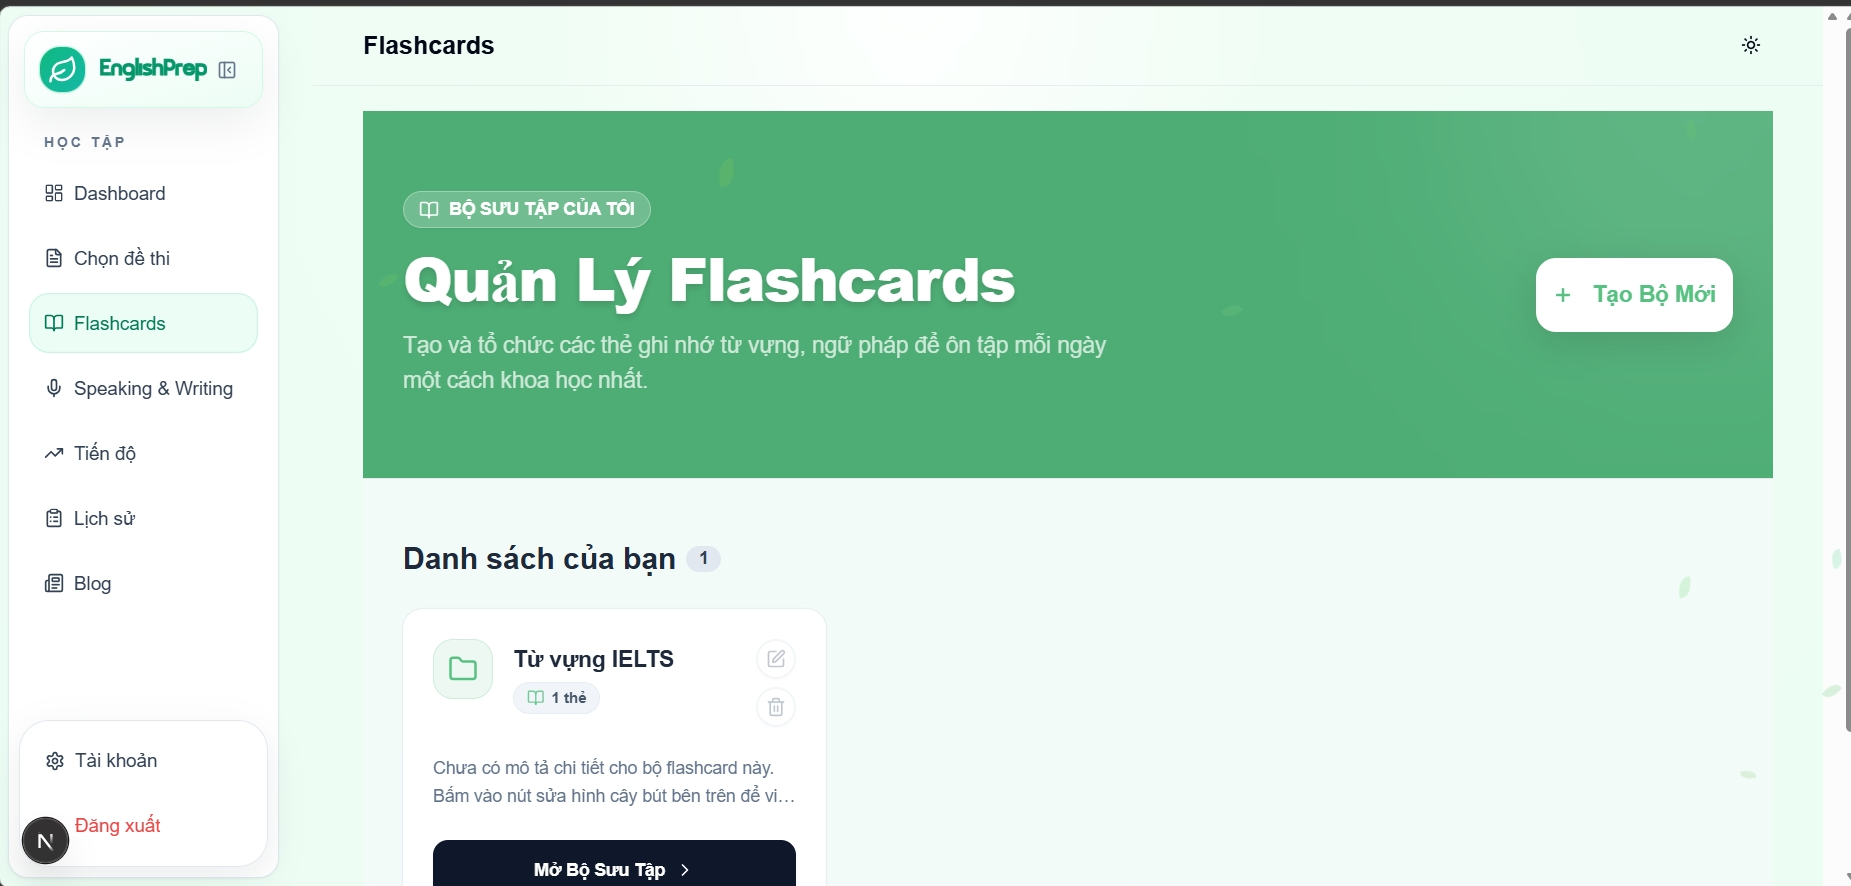
\includegraphics[width=\linewidth]{graphics/ui/flashcard/flashcard-my-list.jpg}
    \captionsetup{skip=5pt}
    \caption{Danh sách bộ flashcard cá nhân}
    \label{h14}
\end{figure}
\noindent Đây là giao diện đầu mối cho hoạt động học từ vựng và ngữ pháp theo phương pháp flashcard trên nền tảng. Thiết kế sử dụng bố cục thanh bên kết hợp không gian làm việc chính để giúp người dùng phân loại nội dung theo từng nhóm học tập hoặc từng kỳ thi cụ thể. Nhờ đó, việc quản lý tài liệu ôn luyện trở nên có tổ chức và dễ mở rộng theo tiến độ học của từng cá nhân.

\begin{figure}[H]
    \centering
    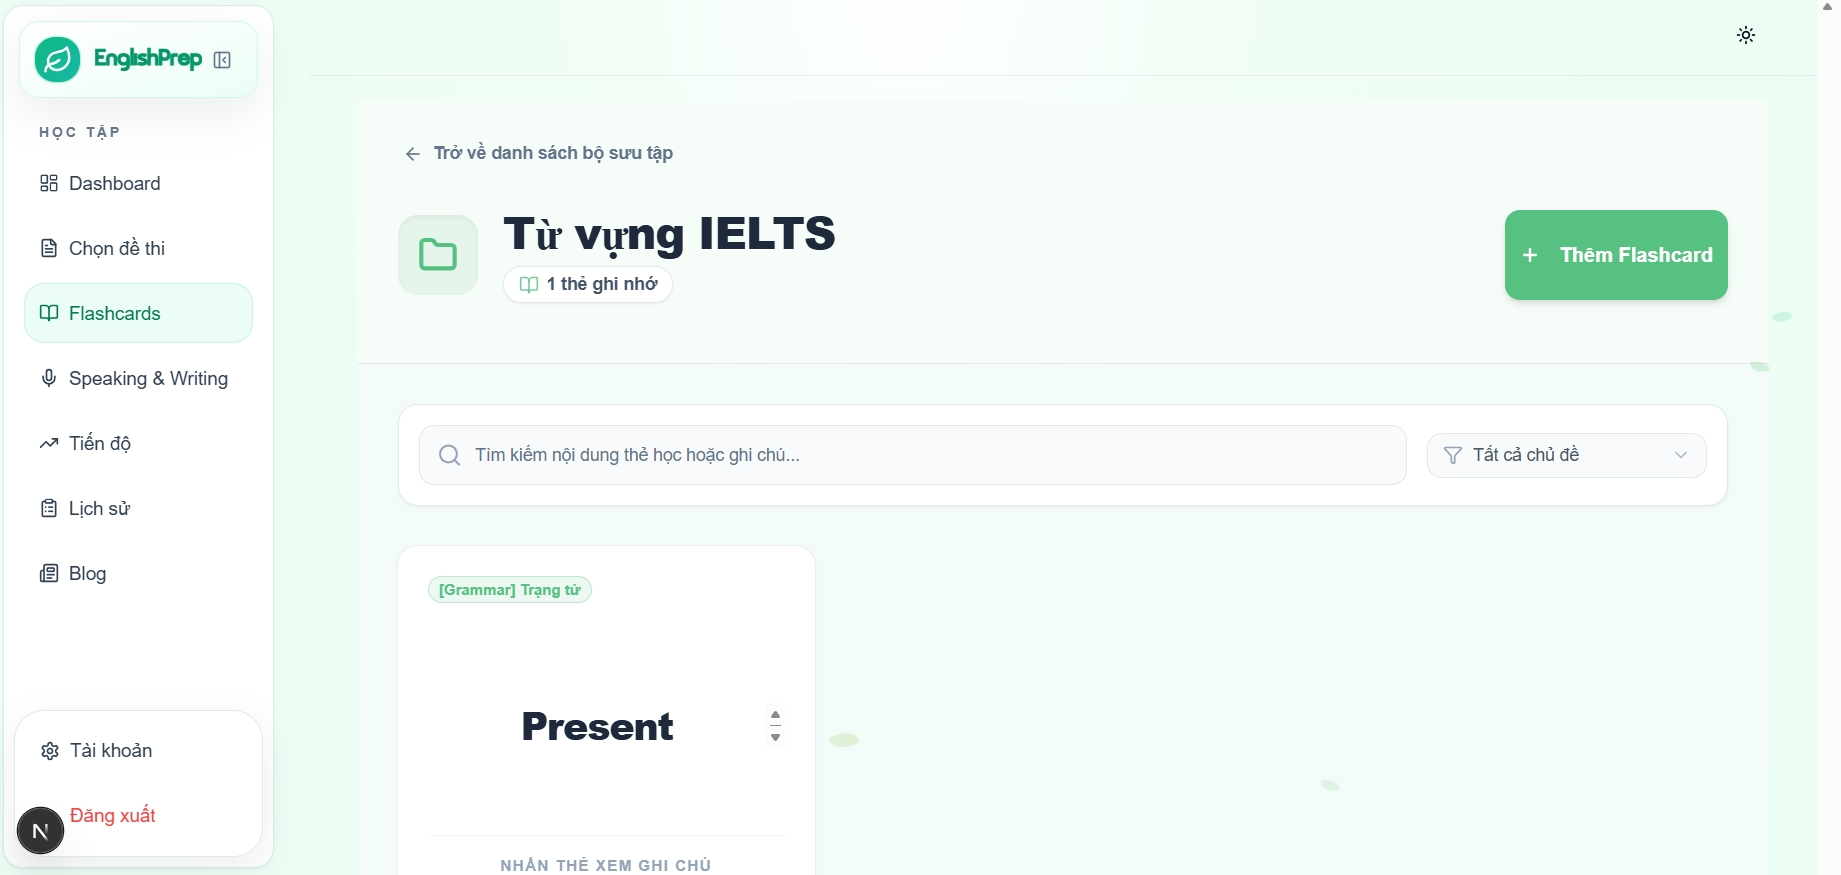
\includegraphics[width=\linewidth]{graphics/ui/flashcard/flashcard-my-flashcard.jpg}
    \captionsetup{skip=5pt}
    \caption{Giao diện học với flashcard}
    \label{h15}
\end{figure}
\noindent Bảng điều khiển flashcard là trung tâm quản lý thư viện ngôn ngữ cá nhân của người học. Bố cục hai cột cân bằng giữa việc hiển thị phân loại tổng quát và quản lý chi tiết từng thẻ, đồng thời được hỗ trợ bởi chức năng tìm kiếm và lọc nội dung. Thiết kế này phù hợp với nhu cầu mở rộng vốn từ vựng theo thời gian mà vẫn giữ cho quá trình tra cứu và ôn tập diễn ra thuận tiện.

\begin{figure}[H]
    \centering
    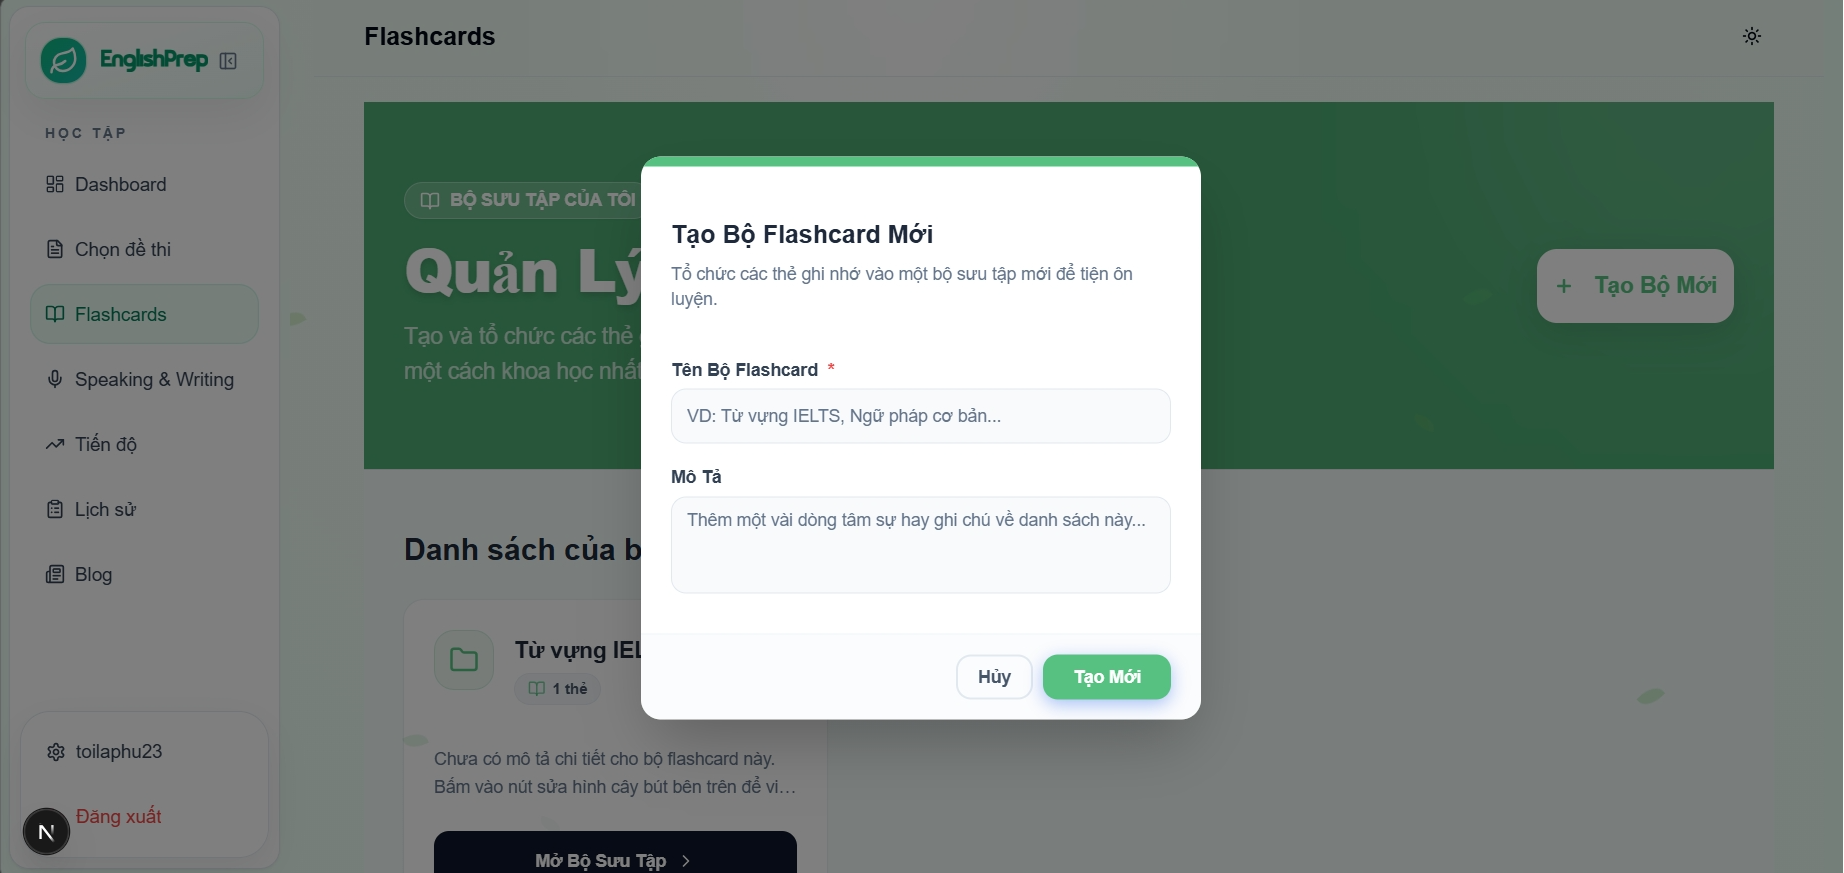
\includegraphics[width=\linewidth]{graphics/ui/flashcard/flashcard-create-list.jpg}
    \captionsetup{skip=5pt}
    \caption{Tạo danh sách flashcard mới}
    \label{h17}
\end{figure}
\noindent Giao diện tạo danh sách mới hỗ trợ người dùng nhóm các tài liệu học thành những bộ có chủ đề riêng biệt. Việc cho phép đặt tên và thêm mô tả chi tiết giúp học viên tổ chức nội dung theo mục tiêu học tập, dạng đề hoặc nhóm từ vựng cụ thể. Điều này góp phần duy trì tính hệ thống và khả năng truy cập nhanh đối với tài liệu ôn luyện.

\begin{figure}[H]
    \centering
    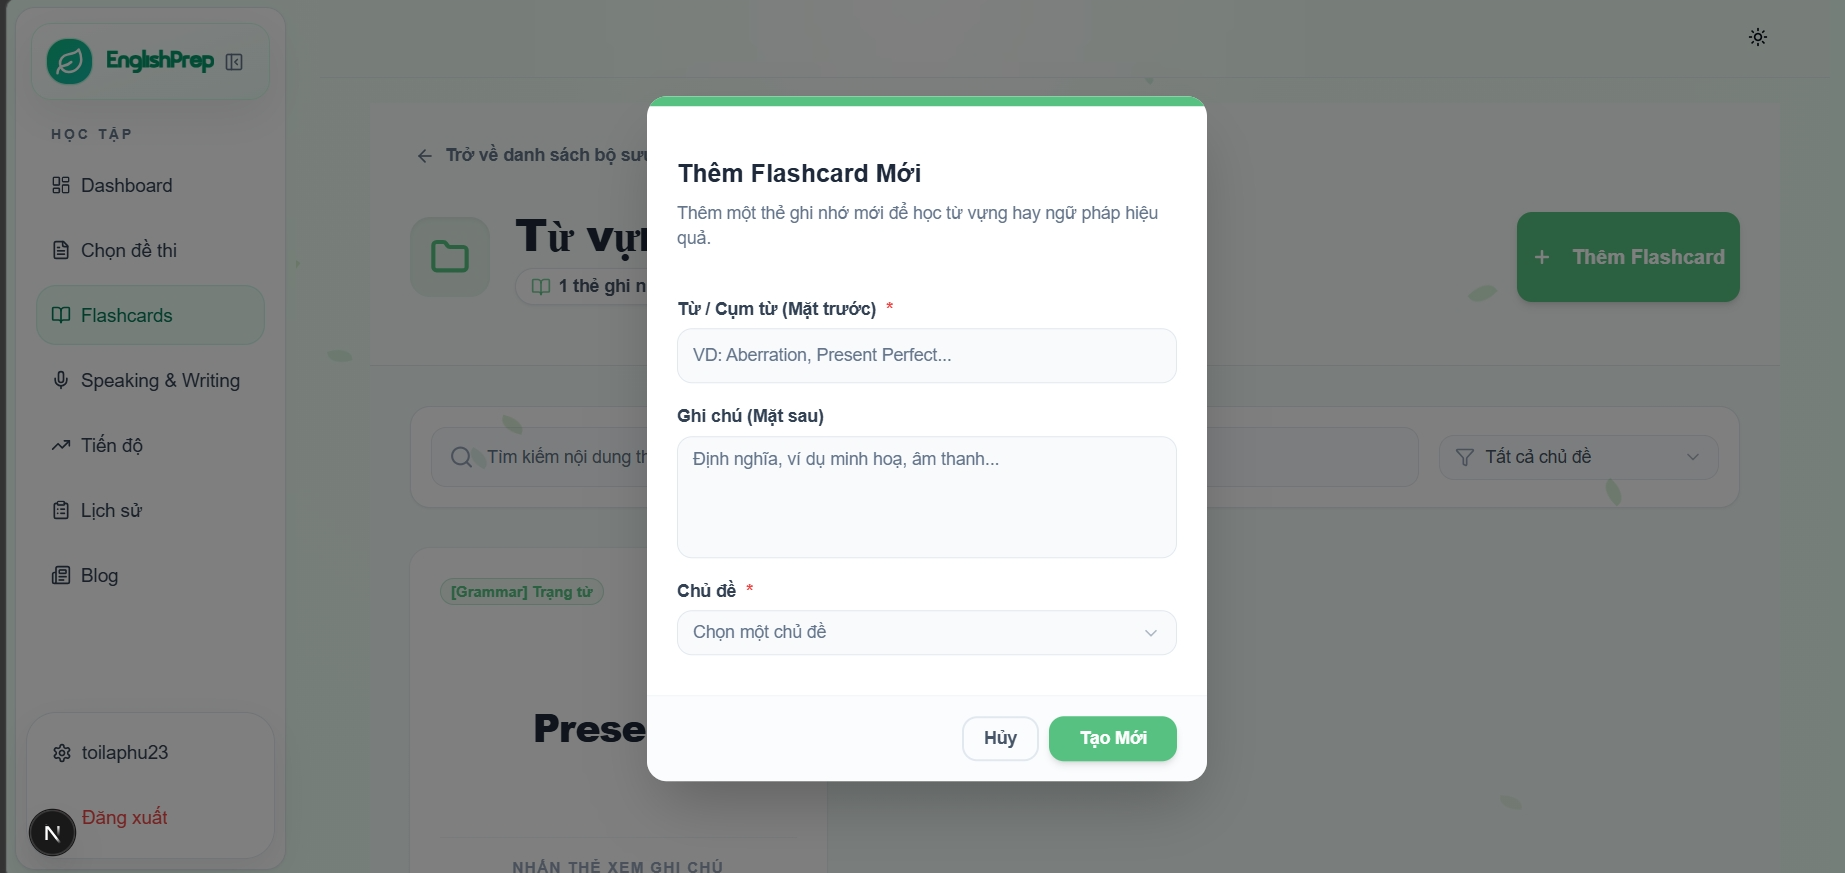
\includegraphics[width=\linewidth]{graphics/ui/flashcard/flashcard-create-flashcard.jpg}
    \captionsetup{skip=5pt}
    \caption{Thêm flashcard mới}
    \label{h18}
\end{figure}
\noindent Hộp thoại thêm flashcard mới là công cụ đơn giản nhưng hiệu quả cho việc tự xây dựng nội dung học tập. Người dùng cần chọn danh sách, chủ đề và nhập thuật ngữ hoặc nội dung ghi nhớ, từ đó bảo đảm rằng hệ thống flashcard luôn được tổ chức nhất quán. Trường ghi chú tùy chọn còn cho phép bổ sung mẹo học, ví dụ hoặc liên tưởng cá nhân để tăng hiệu quả ghi nhớ.

\subsection{Profile}

\begin{figure}[H]
    \centering
    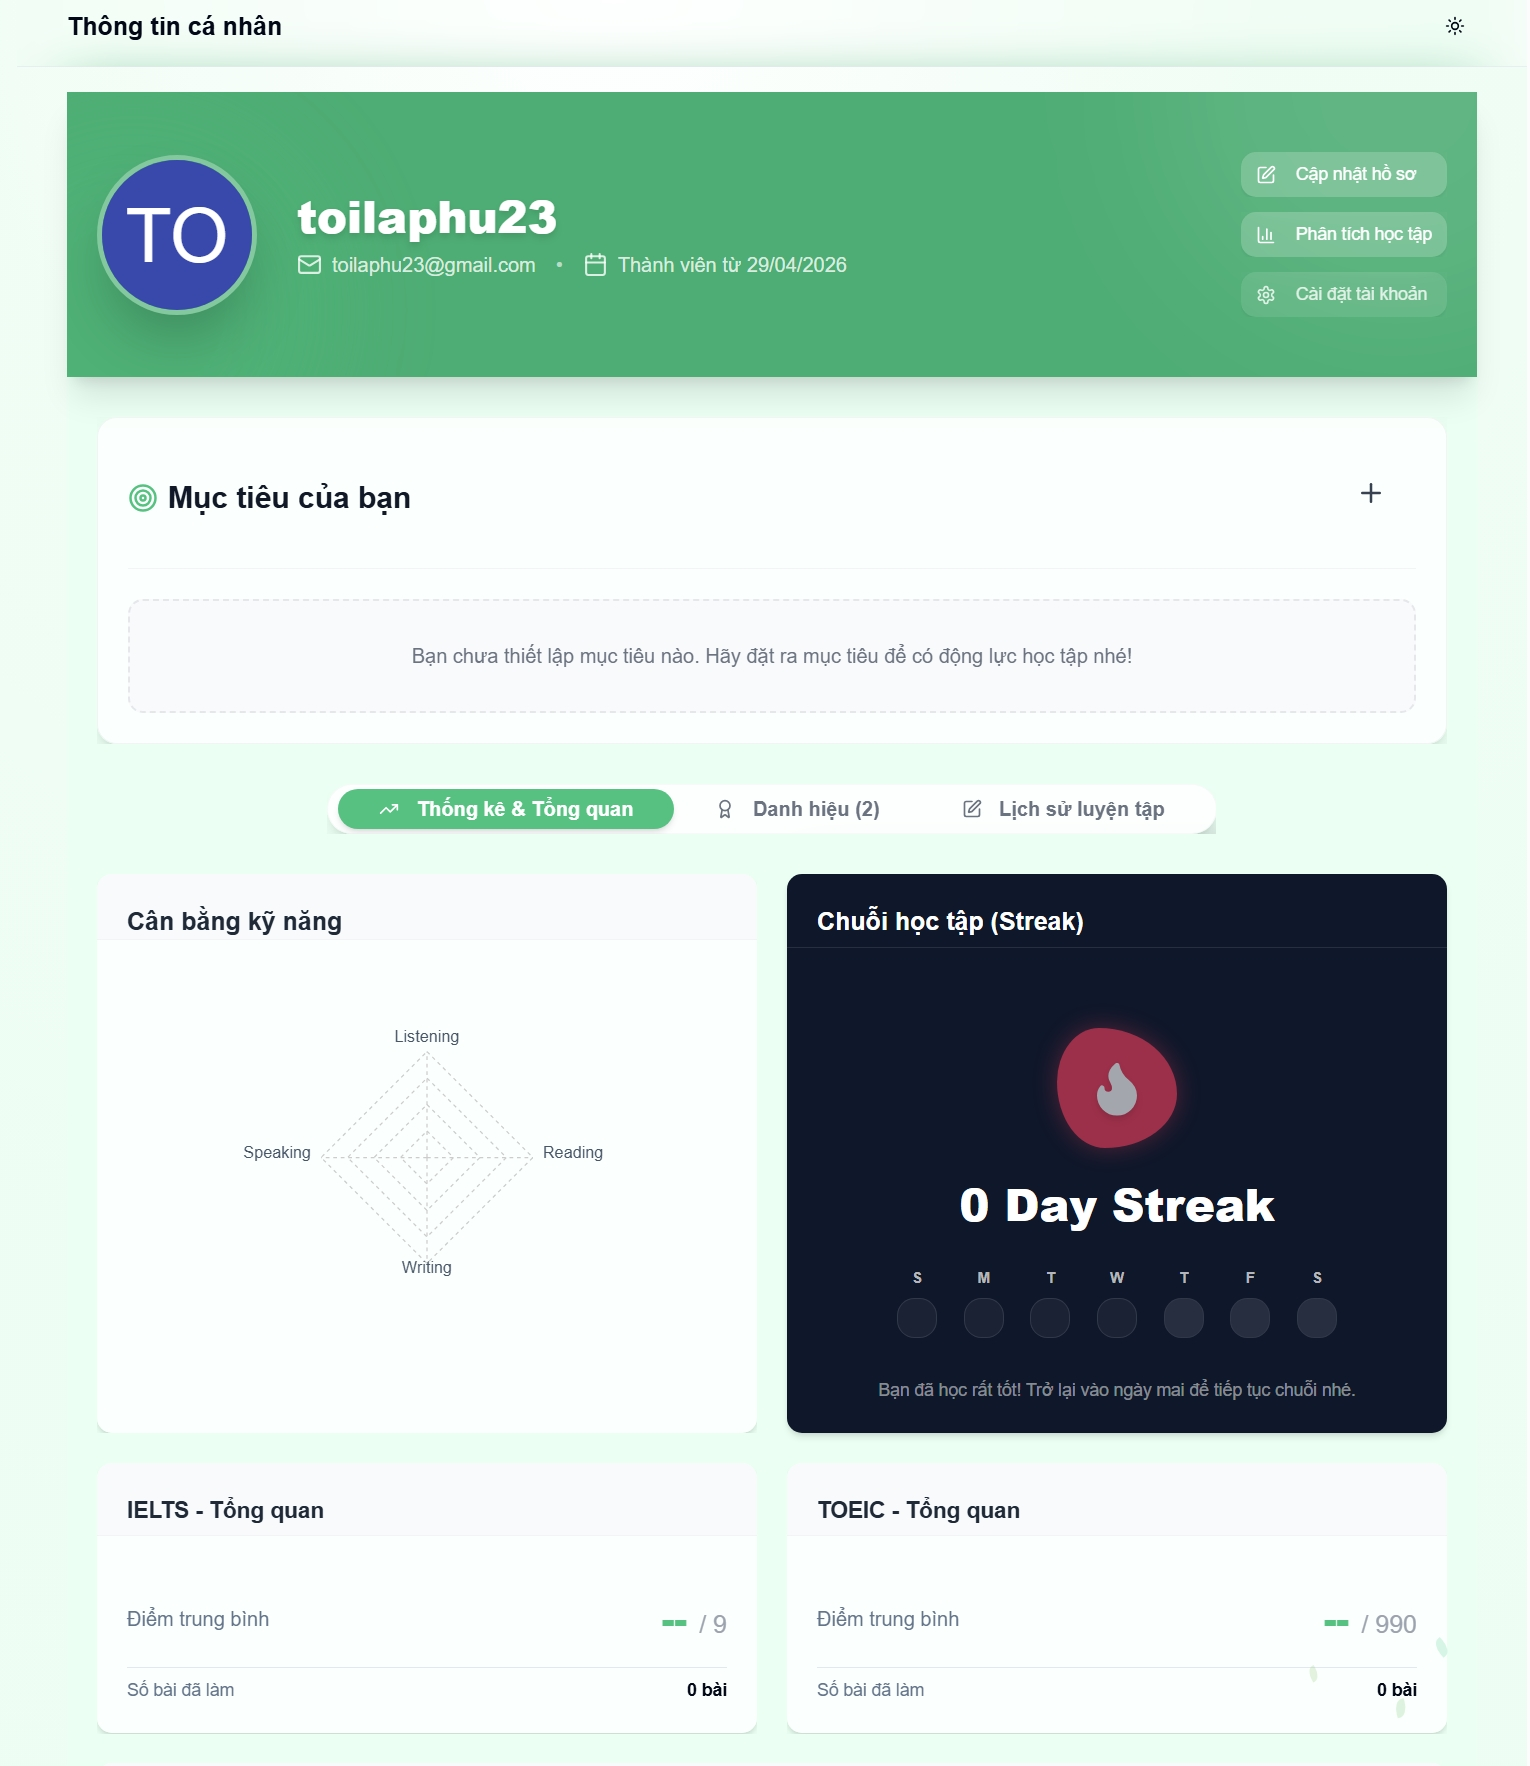
\includegraphics[width=\linewidth]{graphics/ui/profile/profile-overview.jpg}
    \captionsetup{skip=5pt}
    \caption{Tổng quan hồ sơ cá nhân}
\end{figure}
\noindent Giao diện tổng quan hồ sơ cá nhân đóng vai trò như trung tâm theo dõi tiến độ và quản trị tài khoản của người học. Khu vực đầu trang hiển thị ảnh đại diện, tên người dùng, email, ngày tham gia cùng các nút thao tác nhanh như cập nhật hồ sơ, phân tích học tập và cài đặt tài khoản. Ngay bên dưới là khối mục tiêu cá nhân, nơi người dùng theo dõi các cột mốc đã đặt ra hoặc mở hộp thoại để thêm mục tiêu mới. Phần nội dung chính được chia theo các thẻ chức năng; ở thẻ ``Thống kê \& Tổng quan'', hệ thống thể hiện biểu đồ cân bằng kỹ năng, chuỗi học tập và các chỉ số tổng hợp cho IELTS và TOEIC, từ đó hỗ trợ người học nhìn rõ mức độ tiến bộ của mình theo thời gian.

\begin{figure}[H]
    \centering
    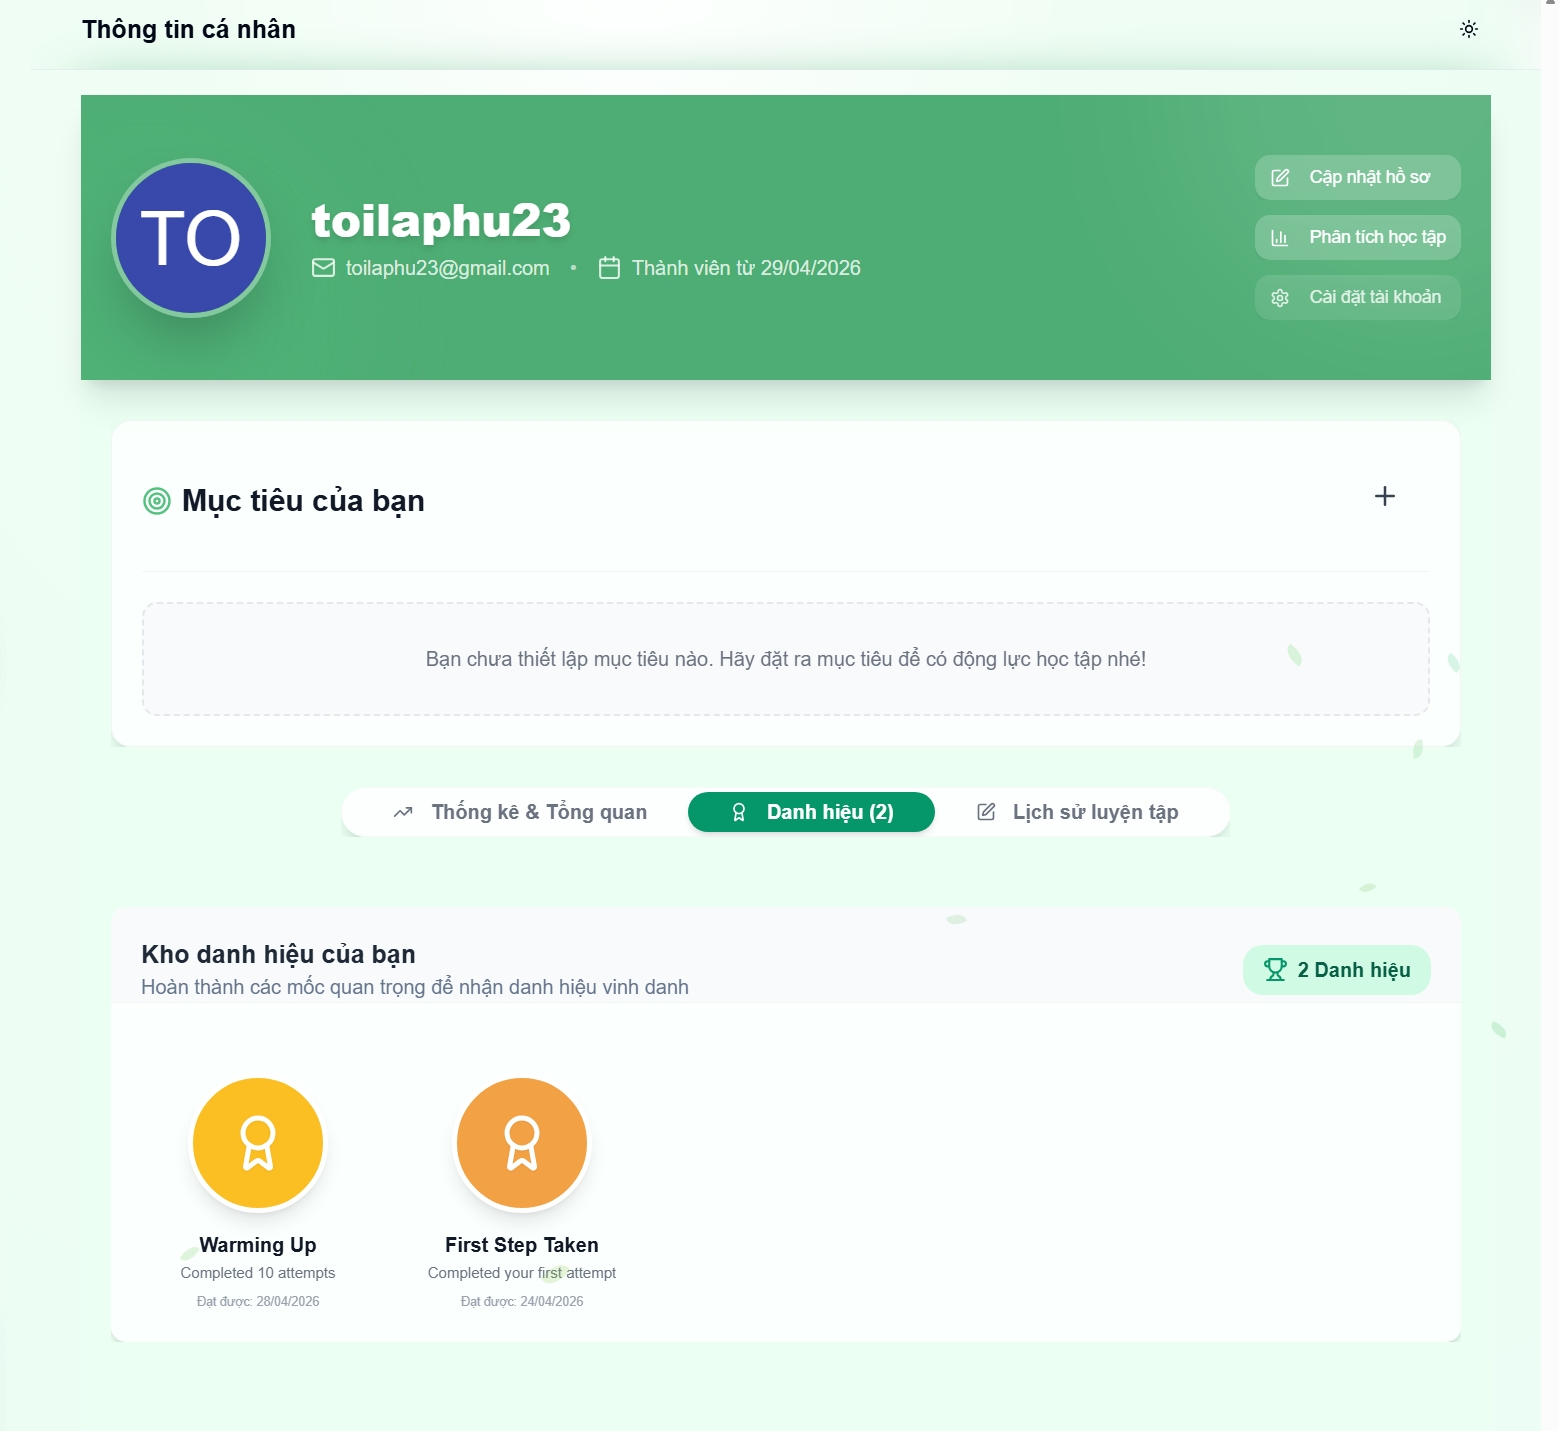
\includegraphics[width=\linewidth]{graphics/ui/profile/profile-achievement.jpg}
    \captionsetup{skip=5pt}
    \caption{Danh hiệu trong hồ sơ cá nhân}
    \label{fig:profile-achievement}
\end{figure}
\noindent Ở thẻ ``Danh hiệu'', hồ sơ cá nhân chuyển trọng tâm từ thống kê sang động lực học tập. Giao diện liệt kê các huy hiệu mà người dùng đã mở khóa, kèm theo tên danh hiệu, điều kiện đạt được và thời điểm nhận thưởng. Cách tổ chức này giúp biến tiến trình luyện tập thành các cột mốc dễ ghi nhớ, đồng thời khuyến khích người học duy trì tần suất làm bài để chinh phục thêm các thành tích mới.

\begin{figure}[H]
    \centering
    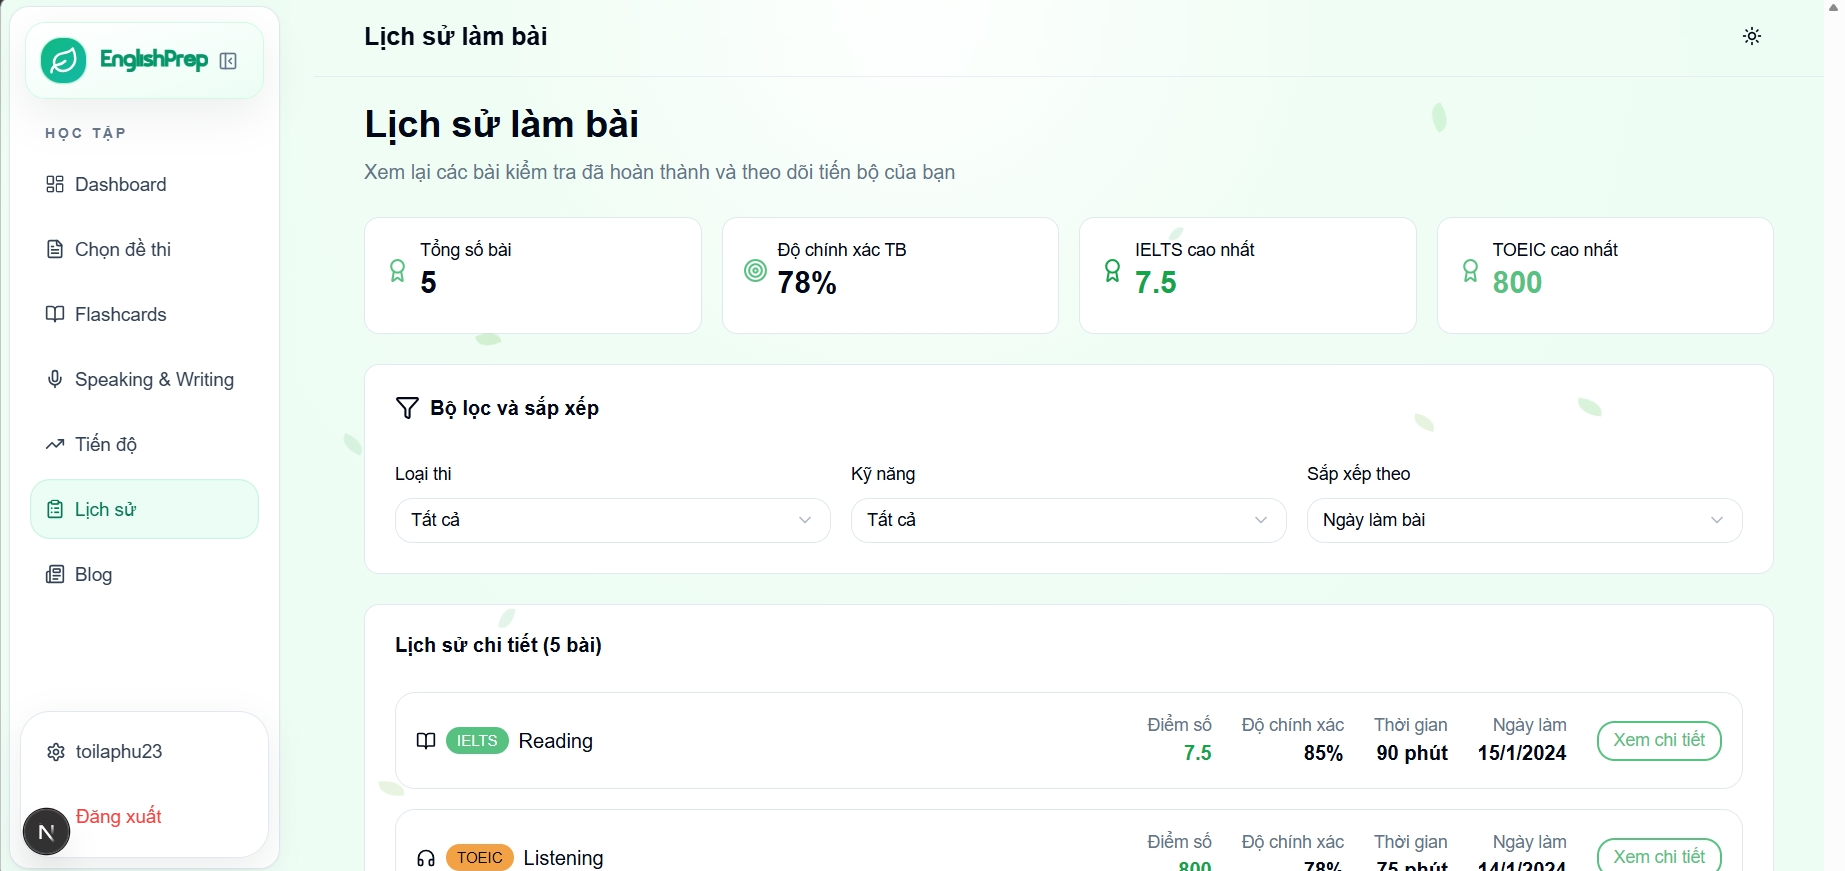
\includegraphics[width=\linewidth]{graphics/ui/profile/profile-history.jpg}
    \captionsetup{skip=5pt}
    \caption{Lịch sử học tập}
    \label{h21}
\end{figure}
\noindent Giao diện lịch sử học tập lưu lại toàn bộ các bài thi và bài luyện mà người dùng đã hoàn thành, qua đó hỗ trợ theo dõi sự tiến bộ theo thời gian. Phần đầu trang hiển thị các chỉ số tổng hợp như tổng số bài đã làm, độ chính xác trung bình, điểm IELTS cao nhất và điểm TOEIC cao nhất. Ngay bên dưới, hệ thống cung cấp bộ lọc theo loại thi, kỹ năng và tiêu chí sắp xếp để người dùng nhanh chóng thu hẹp danh sách cần xem. Mỗi dòng lịch sử đều thể hiện tên bài luyện, loại chứng chỉ, điểm số, độ chính xác, thời gian làm bài và ngày hoàn thành; nút ``Xem chi tiết'' cho phép đi sâu vào từng lần nộp bài để phân tích điểm mạnh, điểm yếu và xu hướng cải thiện.

\begin{figure}[H]
    \centering
    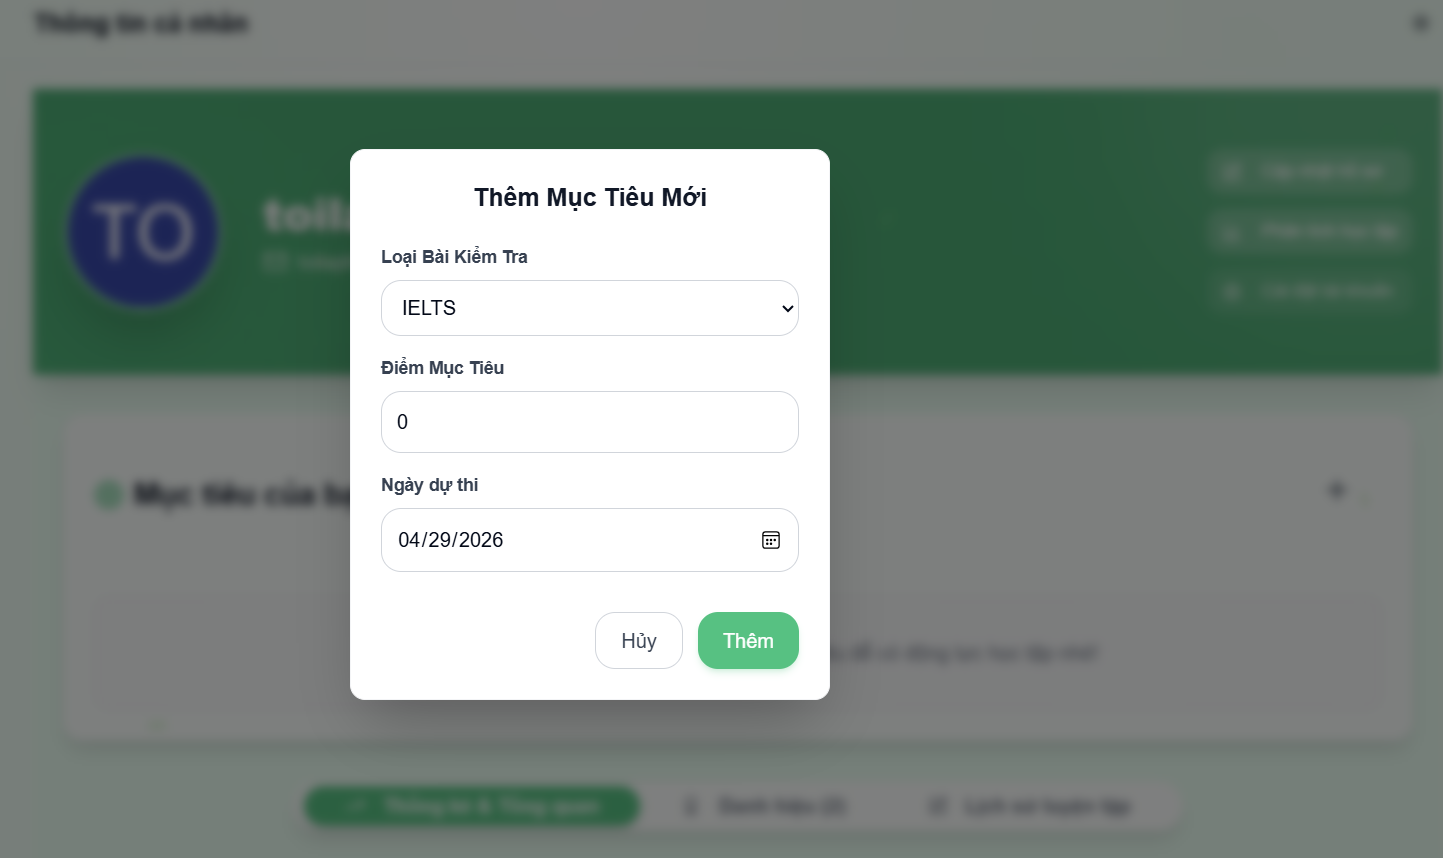
\includegraphics[width=\linewidth]{graphics/ui/profile/profile-add-goal.jpg}
    \captionsetup{skip=5pt}
    \caption{Hộp thoại thiết lập mục tiêu}
    \label{fig:profile-add-goal}
\end{figure}
\noindent Hộp thoại thiết lập mục tiêu cho phép người dùng bổ sung nhanh các cột mốc học tập ngay trong trang hồ sơ mà không cần rời khỏi luồng theo dõi tiến độ. Biểu mẫu tập trung vào các thông tin thiết yếu như tên mục tiêu, loại kỳ thi, điểm mong muốn và thời hạn hoàn thành, giúp việc đặt mục tiêu trở nên rõ ràng và có thể đo lường được. Việc tích hợp thao tác này trực tiếp trong hồ sơ cá nhân giúp người học dễ dàng liên kết kế hoạch dài hạn với dữ liệu luyện tập thực tế đang được hệ thống ghi nhận.

\subsection{Blog}

\begin{figure}[H]
    \centering
    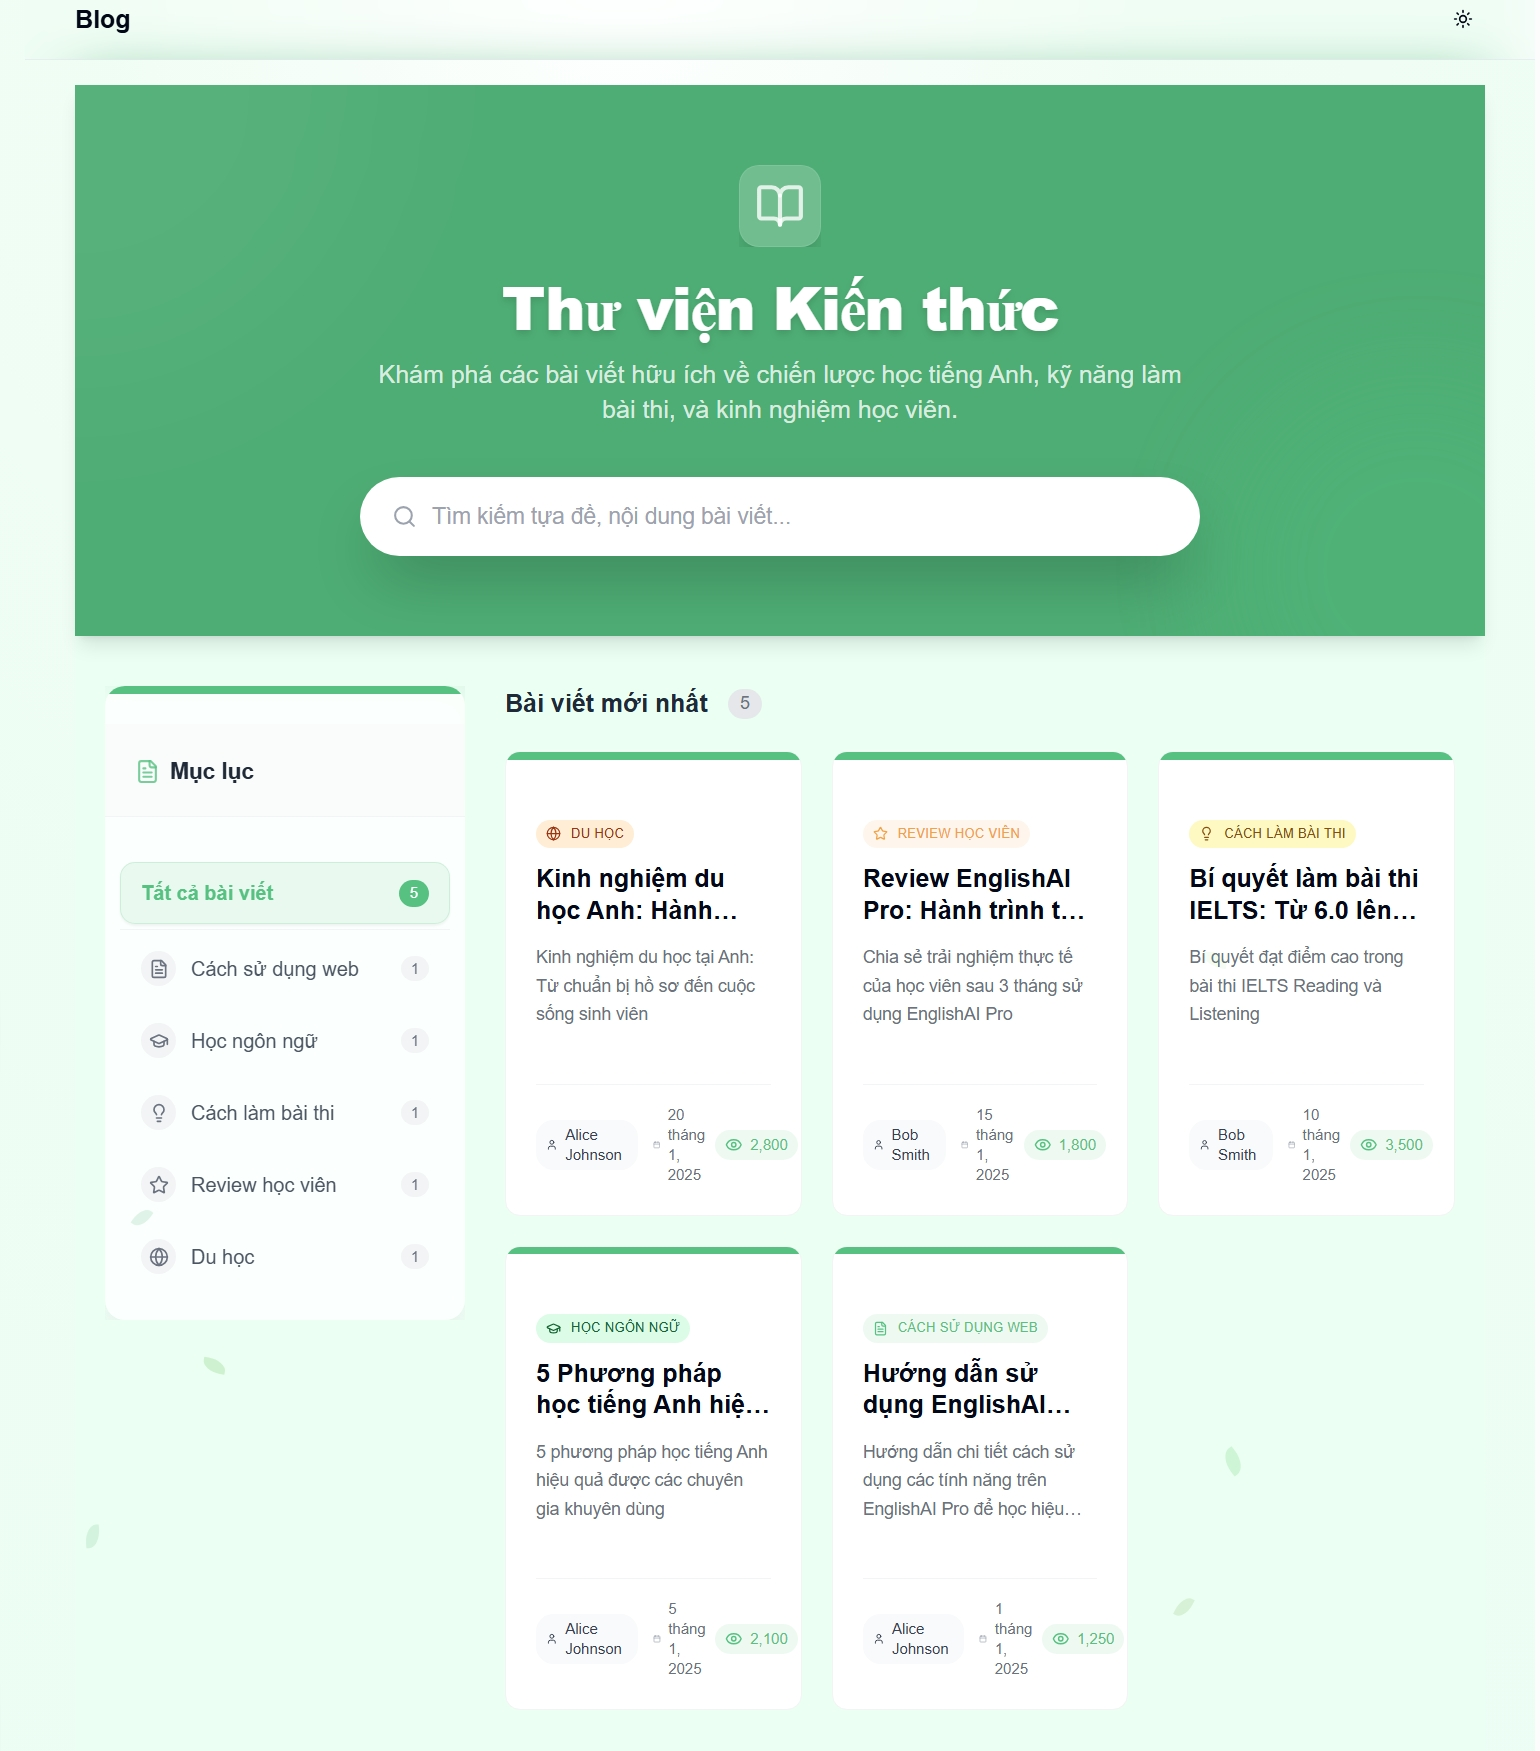
\includegraphics[width=\linewidth]{graphics/ui/blog/blog-selection.jpg}
    \captionsetup{skip=5pt}
    \caption{Danh sách bài viết blog}
    \label{fig:blog-selection}
\end{figure}
\noindent Giao diện blog hoạt động như một trung tâm khám phá nội dung học tập trong hệ thống. Các bài viết được sắp xếp theo dạng lưới dễ quan sát, đi kèm thanh bên hỗ trợ lọc theo chủ đề và các thẻ nội dung tóm tắt thông tin quan trọng của từng bài. Cách tổ chức này giúp người dùng nhanh chóng chuyển đổi giữa các nhóm chủ đề như mẹo luyện thi IELTS, hướng dẫn sử dụng nền tảng hoặc các bài chia sẻ kiến thức liên quan.

\begin{figure}[H]
    \centering
    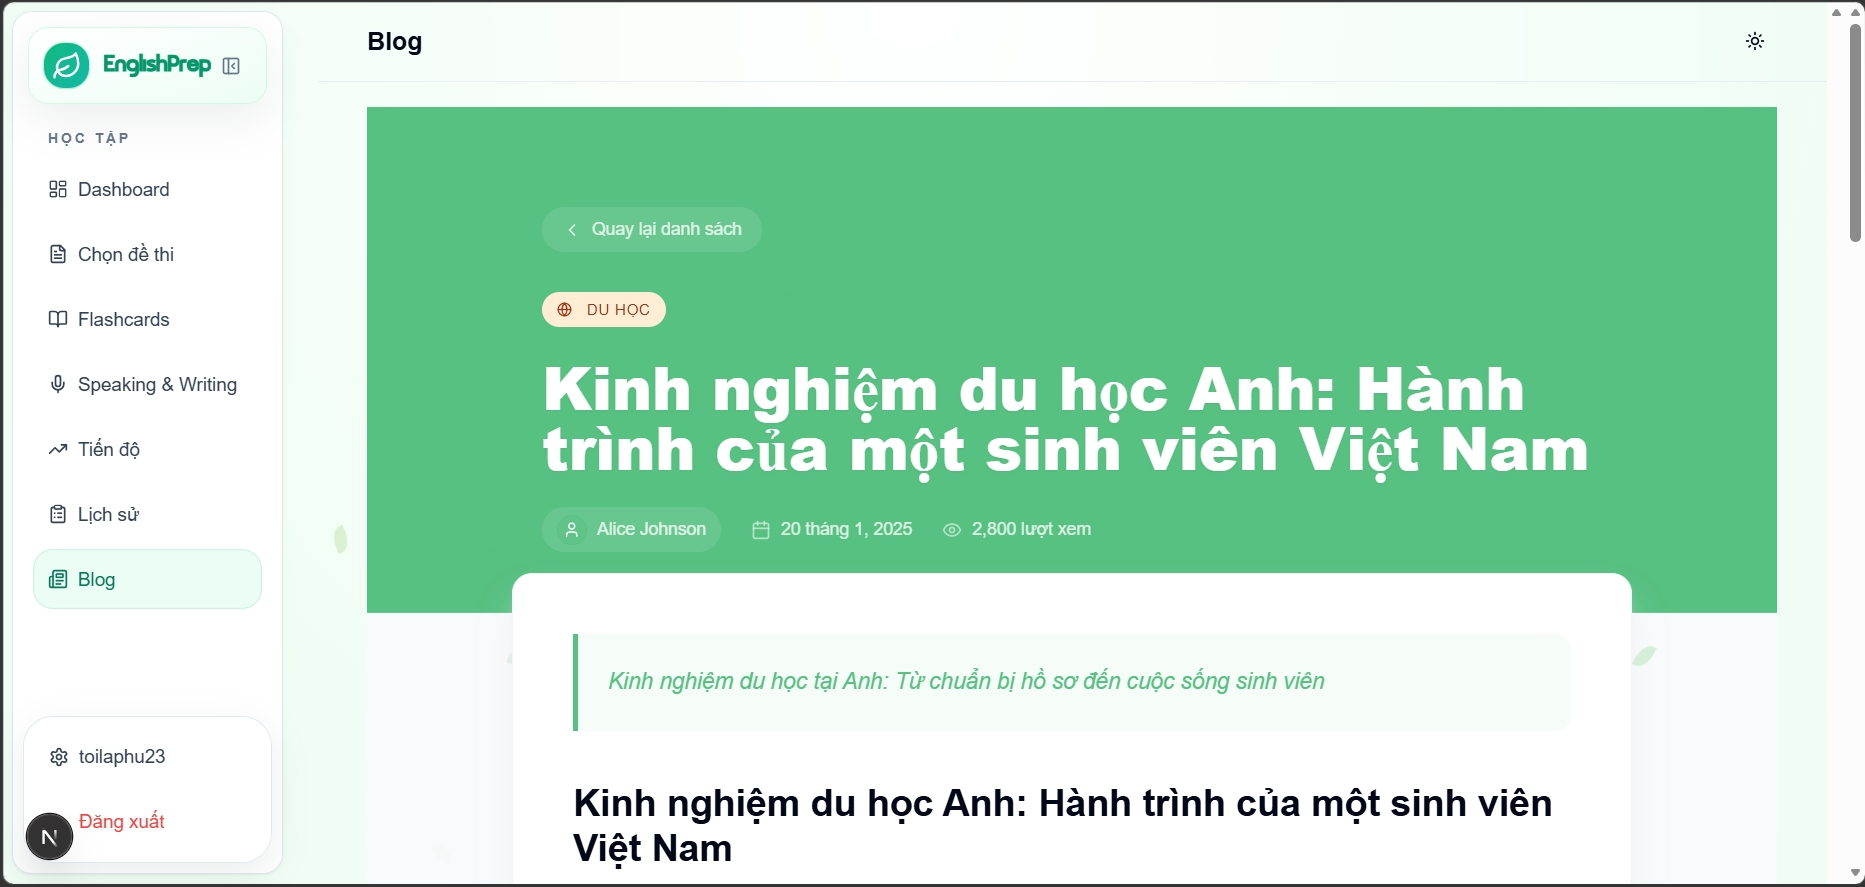
\includegraphics[width=\linewidth]{graphics/ui/blog/blog-example.jpg}
    \captionsetup{skip=5pt}
    \caption{Trang chi tiết bài viết blog}
    \label{fig:blog-example}
\end{figure}
\noindent Trang hiển thị bài viết blog được thiết kế theo hướng dễ đọc và chuyên nghiệp. Quản trị viên hoặc người tạo nội dung có thể trình bày bài viết bằng cấu trúc phân cấp gồm tiêu đề, đề mục và danh sách gạch đầu dòng để truyền tải thông tin dài một cách rõ ràng. Sự kết hợp giữa điều hướng tiêu chuẩn, thông tin bài viết và nội dung chính giúp tạo nên trải nghiệm đọc mạch lạc và hấp dẫn đối với người dùng.

\subsection{Admin Dashboard}

\begin{figure}[H]
    \centering
    \IfFileExists{graphics/ui/admin/exam-creation.jpg}{%
        
\includegraphics[width=\linewidth]{graphics/ui/admin/exam-creation.jpg}%
    }{%
        \fbox{\parbox[c][0.3\textheight][c]{0.9\linewidth}{\centering Placeholder cho giao diện tạo đề thi\newline (chưa có tệp hình trong thư mục graphics/ui/admin)}}%
    }
    \captionsetup{skip=5pt}
    \caption{Giao diện tạo đề thi}
    \label{fig:admin-exam-creation}
\end{figure}

\noindent Giao diện tạo đề thi là không gian làm việc chuyên biệt dành cho quản trị viên khi xây dựng nội dung luyện tập mới trên hệ thống. Quản trị viên có thể tổ chức cấu trúc đề thi thông qua thanh điều hướng phân cấp, đồng thời nhập văn bản, tải lên phương tiện và tạo các câu hỏi chi tiết cho từng phần. Hệ thống cũng cho phép lựa chọn loại câu hỏi và số điểm tương ứng, từ đó hỗ trợ số hóa nội dung giáo dục theo quy trình chặt chẽ và nhất quán. Các nút hành động ở phần đầu và cuối trang giúp việc lưu tiến độ hoặc di chuyển giữa các mục trở nên thuận tiện hơn.

\begin{figure}[H]
    \centering
    \IfFileExists{graphics/ui/admin/exam-approval.jpg}{%
        
\includegraphics[width=\linewidth]{graphics/ui/admin/exam-approval.jpg}%
    }{%
        \fbox{\parbox[c][0.3\textheight][c]{0.9\linewidth}{\centering Placeholder cho giao diện phê duyệt đề thi\newline (chưa có tệp hình trong thư mục graphics/ui/admin)}}%
    }
    \captionsetup{skip=5pt}
    \caption{Giao diện phê duyệt đề thi}
    \label{fig:admin-exam-approval}
\end{figure}

\noindent Trang phê duyệt đề thi là khu vực làm việc tập trung dành cho quản trị viên cấp cao hoặc người kiểm duyệt nội dung. Giao diện ưu tiên khả năng quan sát với các thống kê tổng quan và bảng dữ liệu chứa những thông tin quan trọng như loại đề, độ khó và người tạo. Dựa trên đó, quản trị viên có thể nhanh chóng phê duyệt hoặc từ chối các đề thi đang chờ xử lý. Nếu cần xem xét sâu hơn, người quản trị có thể nhấp vào tên đề để chuyển đến trang chỉnh sửa chi tiết. Quy trình này góp phần bảo đảm chất lượng học liệu và duy trì tính nhất quán cho toàn bộ hệ thống.

\section{LingriserSpeaking}

Phần này trình bày các giao diện tiêu biểu của \textit{LingriserSpeaking}, mô-đun luyện nói tiếng Anh tích hợp AI được phát triển song song với nền tảng chính. Khác với nhóm wireframe trước đó vốn tập trung vào hệ thống luyện thi IELTS và TOEIC tổng quát, các màn hình trong LingriserSpeaking được tổ chức xoay quanh chu trình học tập theo tuần, phối hợp giữa học sinh, phụ huynh, mentor và quản trị viên. Các giao diện dưới đây cho thấy cách hệ thống hỗ trợ từ giai đoạn định hướng chương trình, luyện nói với AI, đặt lịch học đồng bộ cho đến theo dõi tiến độ và vận hành toàn bộ nền tảng.

\subsection{Student Dashboard}

\begin{figure}[H]
    \centering
    
\includegraphics[width=\linewidth]{graphics/lingriser/dashboard.png}
    \captionsetup{skip=5pt}
    \caption{Bảng điều khiển học sinh trong LingriserSpeaking}
    \label{fig:lingriser-student-dashboard}
\end{figure}
\noindent Dashboard học sinh là điểm điều phối trung tâm của toàn bộ trải nghiệm luyện nói trên LingriserSpeaking. Bố cục của màn hình ưu tiên việc tóm tắt nhanh module hiện tại, các buổi học sắp tới, mức độ luyện tập với AI và tiến trình của chương trình học theo tuần. Các khối nội dung được sắp xếp theo hướng giúp người học nhìn thấy ngay mình đang ở đâu trong lộ trình, cần hoàn thành hoạt động nào tiếp theo và đâu là những dữ liệu quan trọng như video tiến độ hoặc lịch học đồng bộ. Nhờ đó, dashboard không chỉ đóng vai trò hiển thị thông tin mà còn trở thành điểm xuất phát tự nhiên cho các phiên luyện nói hằng ngày.

\subsection{Mentor Booking}

\begin{figure}[H]
    \centering
    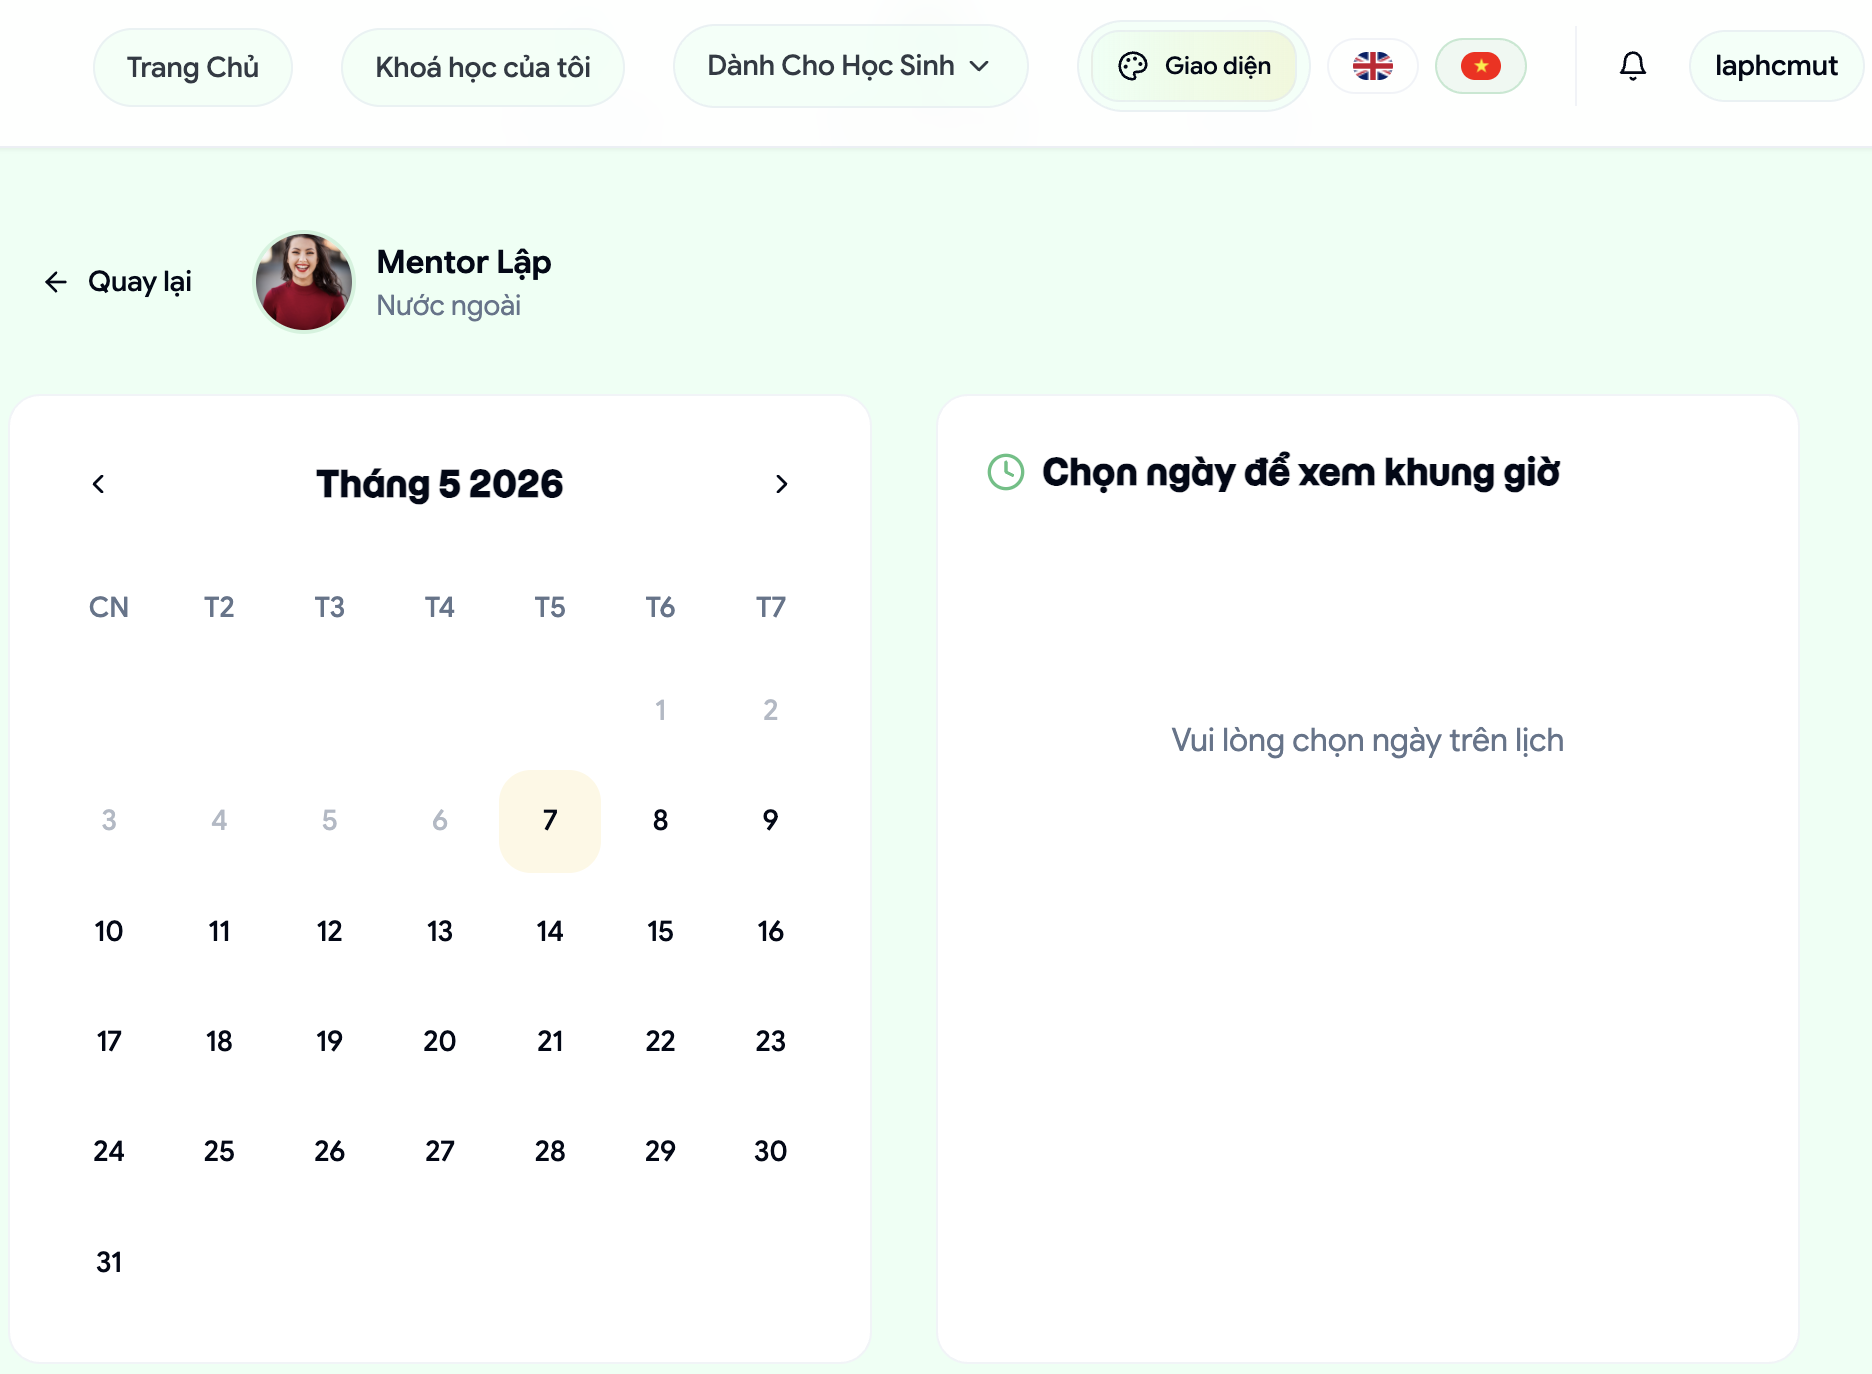
\includegraphics[width=0.9\linewidth]{graphics/lingriser/mentor.png}
    \captionsetup{skip=5pt}
    \caption{Giao diện lựa chọn mentor và đặt lịch video call}
    \label{fig:lingriser-mentor-booking}
\end{figure}
\noindent Giao diện làm việc với mentor tập trung vào hai nhu cầu chính: lựa chọn người hướng dẫn phù hợp và chốt lịch học vào các khung giờ khả dụng. Màn hình kết hợp phần thông tin hồ sơ mentor với khu vực lịch hoặc các phiên học để người dùng có thể so sánh, theo dõi tình trạng trống và thực hiện đặt lịch ngay trong cùng một luồng thao tác. Cách tổ chức này làm giảm độ phân mảnh của trải nghiệm, giúp việc chuyển từ luyện nói bất đồng bộ với AI sang buổi học đồng bộ với người thật diễn ra mạch lạc hơn. Đồng thời, giao diện cũng góp phần làm rõ vai trò của mentor như một tác nhân tiếp nối trực tiếp kết quả luyện tập trong tuần.

\subsection{Parent Dashboard}

\begin{figure}[H]
    \centering
    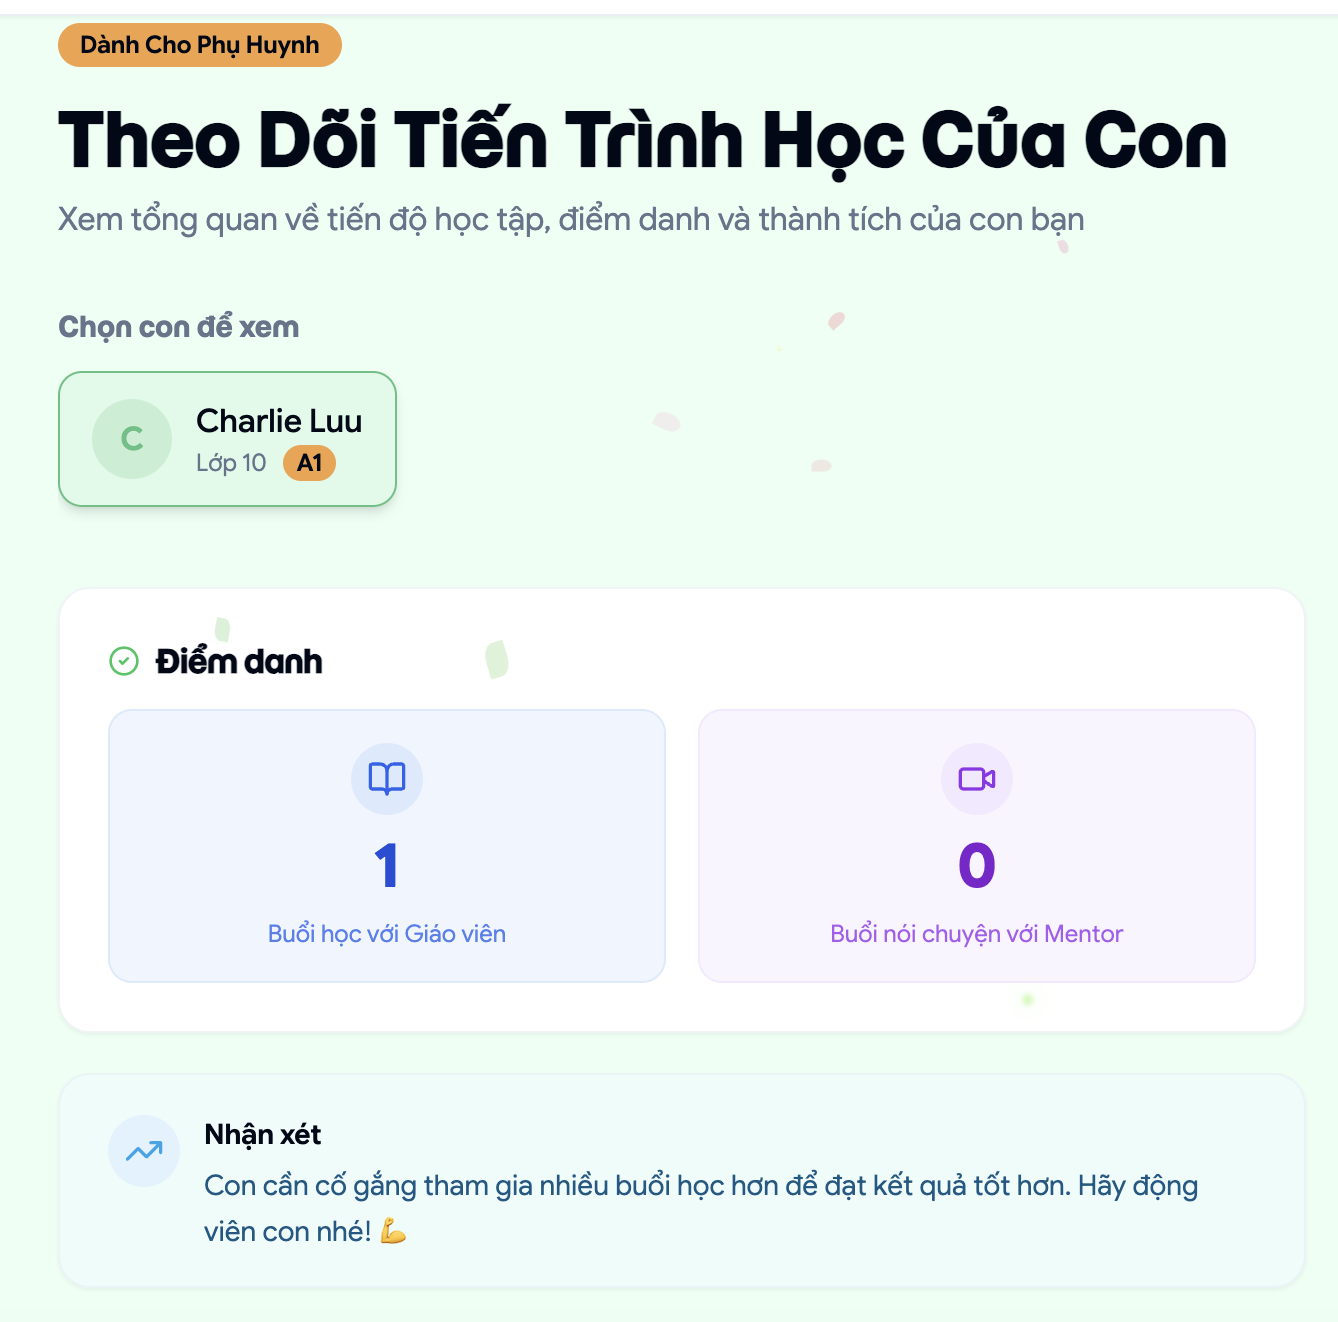
\includegraphics[width=0.88\linewidth]{graphics/lingriser/parents.png}
    \captionsetup{skip=5pt}
    \caption{Bảng điều khiển phụ huynh theo dõi tiến trình học tập}
    \label{fig:lingriser-parent-dashboard}
\end{figure}
\noindent Dashboard phụ huynh được thiết kế như một không gian quan sát tiến trình học tập của con thay vì một khu vực thao tác học trực tiếp. Giao diện ưu tiên các thành phần tổng hợp như thông tin học sinh, mức độ tham gia, lịch học, hoạt động gần đây và các chỉ báo tiến bộ để phụ huynh có thể nhanh chóng nắm bắt tình hình chung. Việc đưa dữ liệu AI practice, lịch sử học tập và video tiến độ vào cùng một màn hình giúp phụ huynh theo dõi sự thay đổi của người học theo thời gian mà không cần truy cập vào nhiều trang riêng lẻ. Đây là một điểm khác biệt quan trọng của LingriserSpeaking khi mở rộng giá trị của dữ liệu luyện nói sang cả bối cảnh đồng hành từ gia đình.

\subsection{Programs}

\begin{figure}[H]
    \centering
    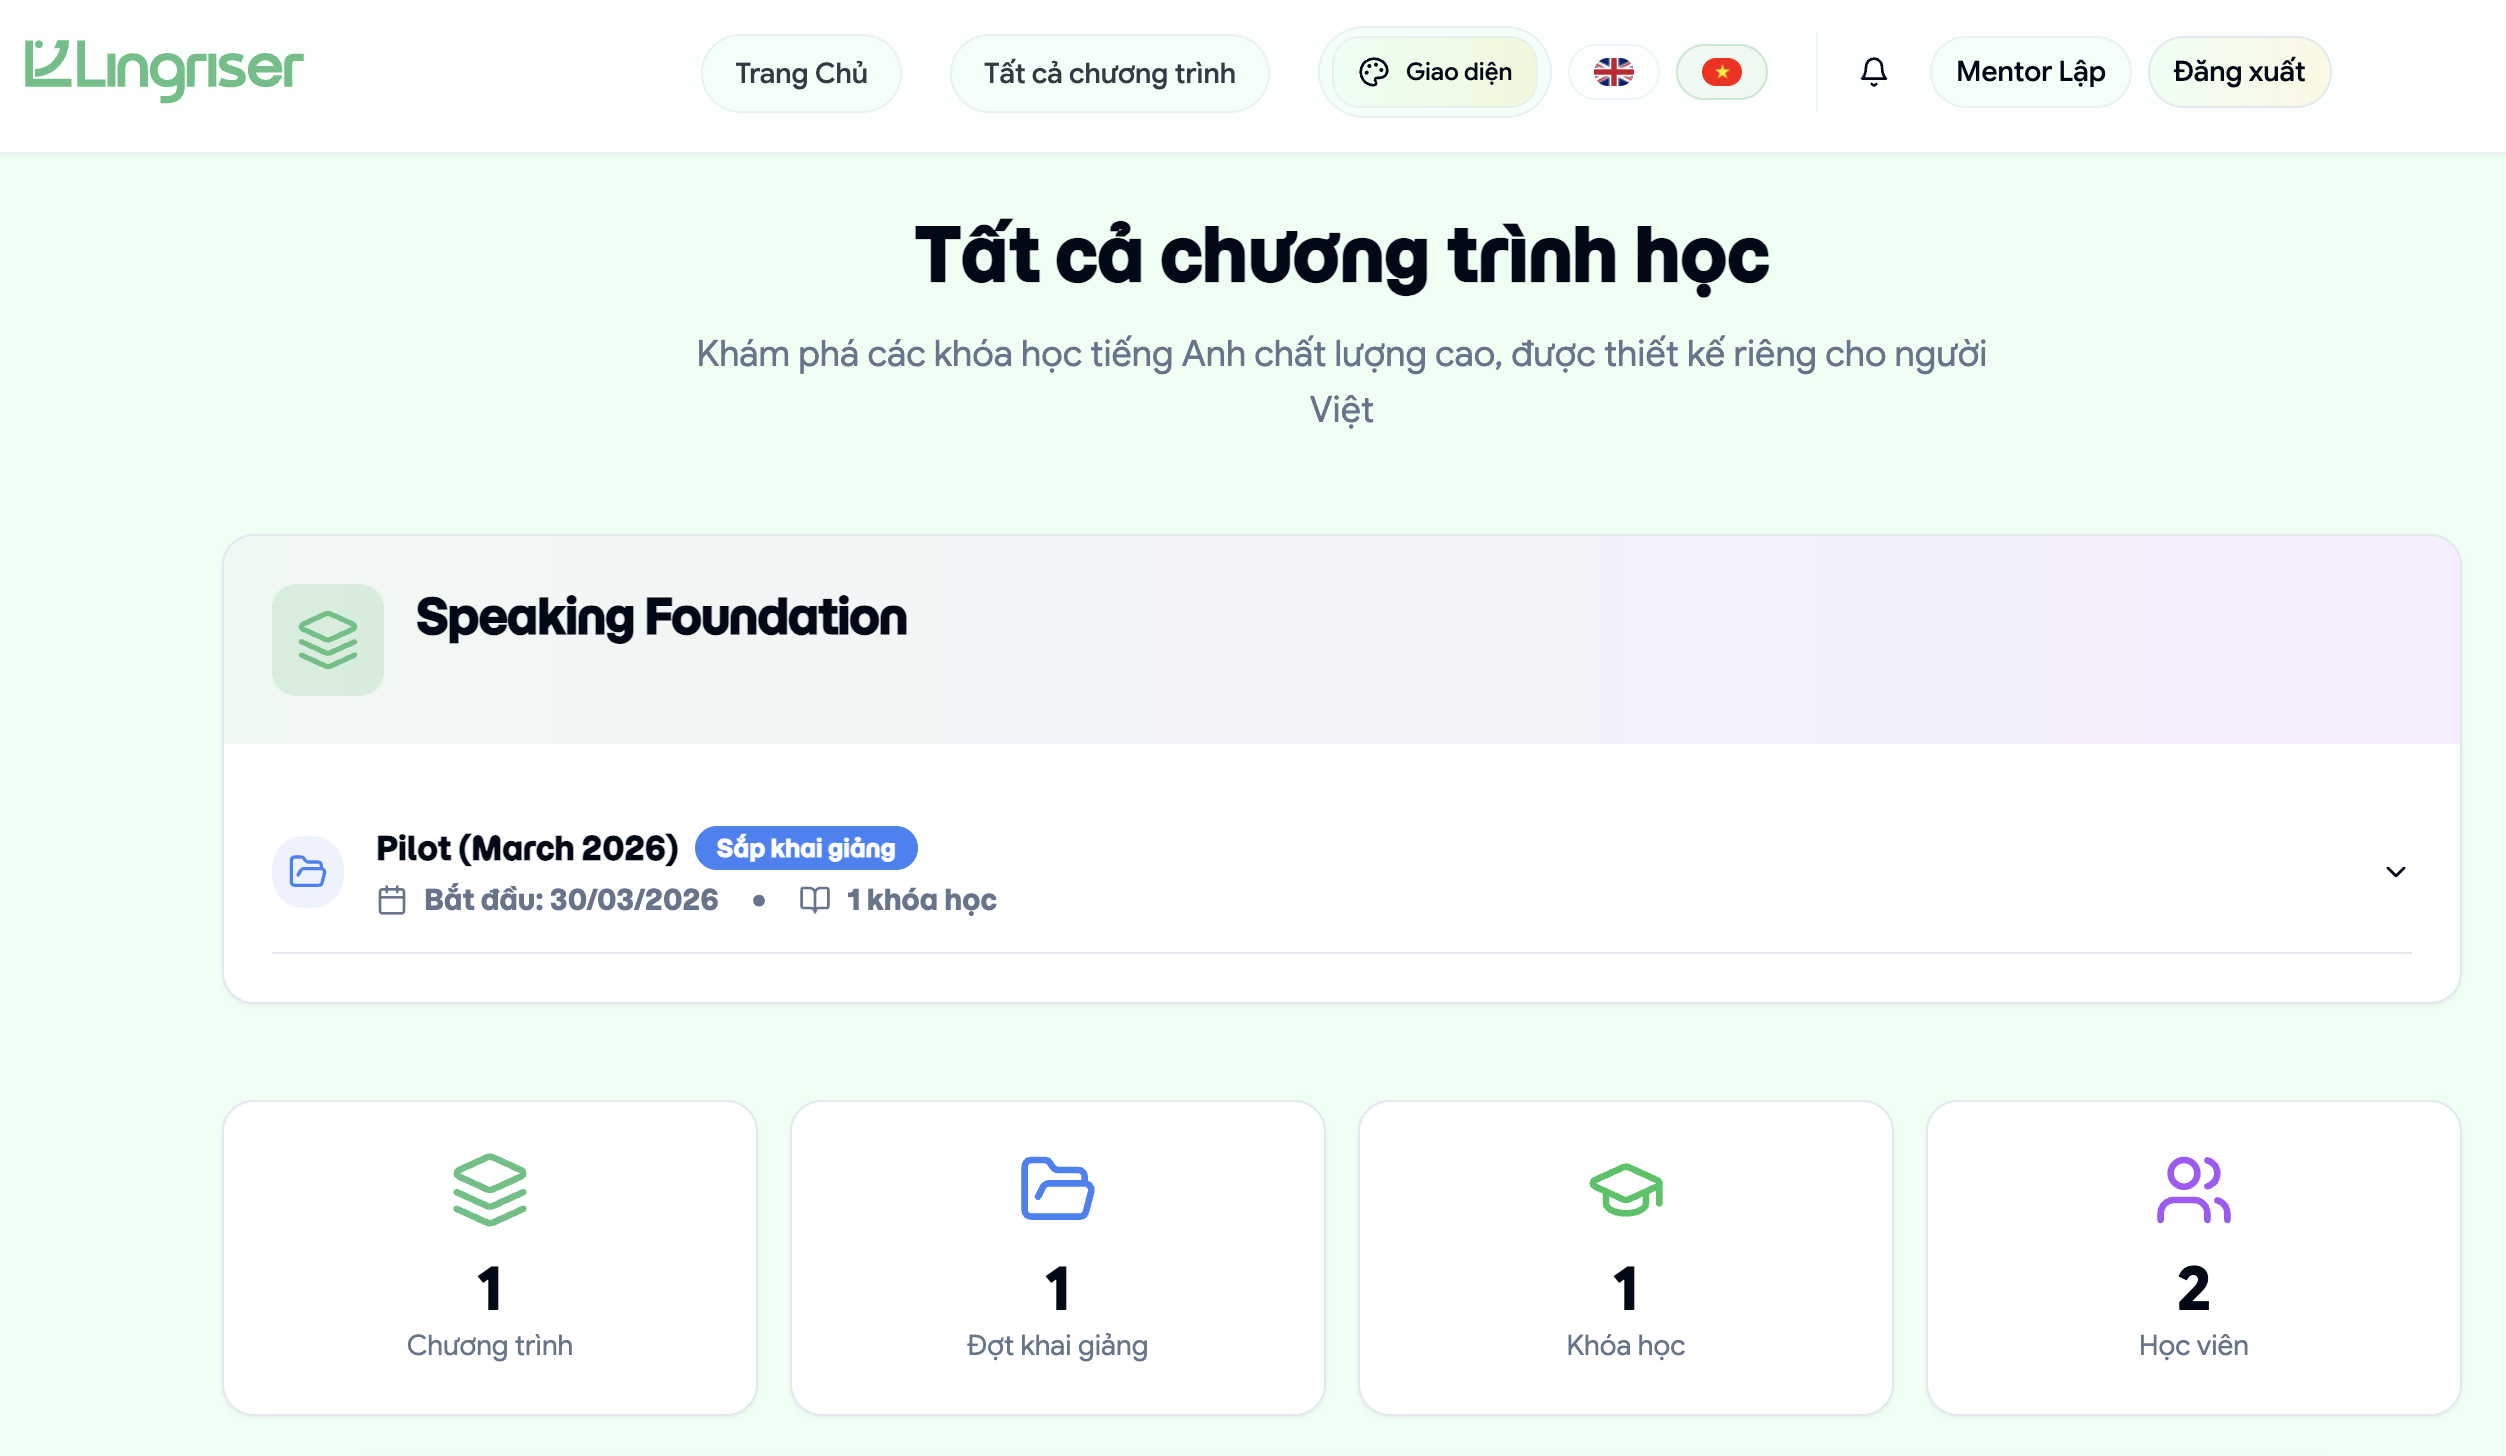
\includegraphics[width=0.9\linewidth]{graphics/lingriser/programs.png}
    \captionsetup{skip=5pt}
    \caption{Giao diện quản lý chương trình học và tiến trình theo mô-đun}
    \label{fig:lingriser-programs}
\end{figure}
\noindent Trang chương trình học trình bày cấu trúc đào tạo của LingriserSpeaking theo hướng phân cấp rõ ràng giữa chương trình, nhóm học, khóa học và các mô-đun. Nhờ cách bố trí này, người dùng hoặc quản trị viên có thể theo dõi được mối quan hệ giữa nội dung học, tiến độ mở khóa và trạng thái tham gia của từng học viên. Giao diện không chỉ hỗ trợ quan sát tổng thể mà còn giúp định vị chính xác vị trí của người học trong lộ trình 8 tuần, từ đó tạo nền tảng cho việc gắn mục tiêu tuần, đặt lịch với mentor và lưu lịch sử luyện tập theo từng giai đoạn. Về mặt thiết kế thông tin, đây là màn hình giữ vai trò liên kết giữa cấu trúc học thuật và các hoạt động Speaking diễn ra hằng ngày.

\subsection{Admin Dashboard}

\begin{figure}[H]
    \centering
    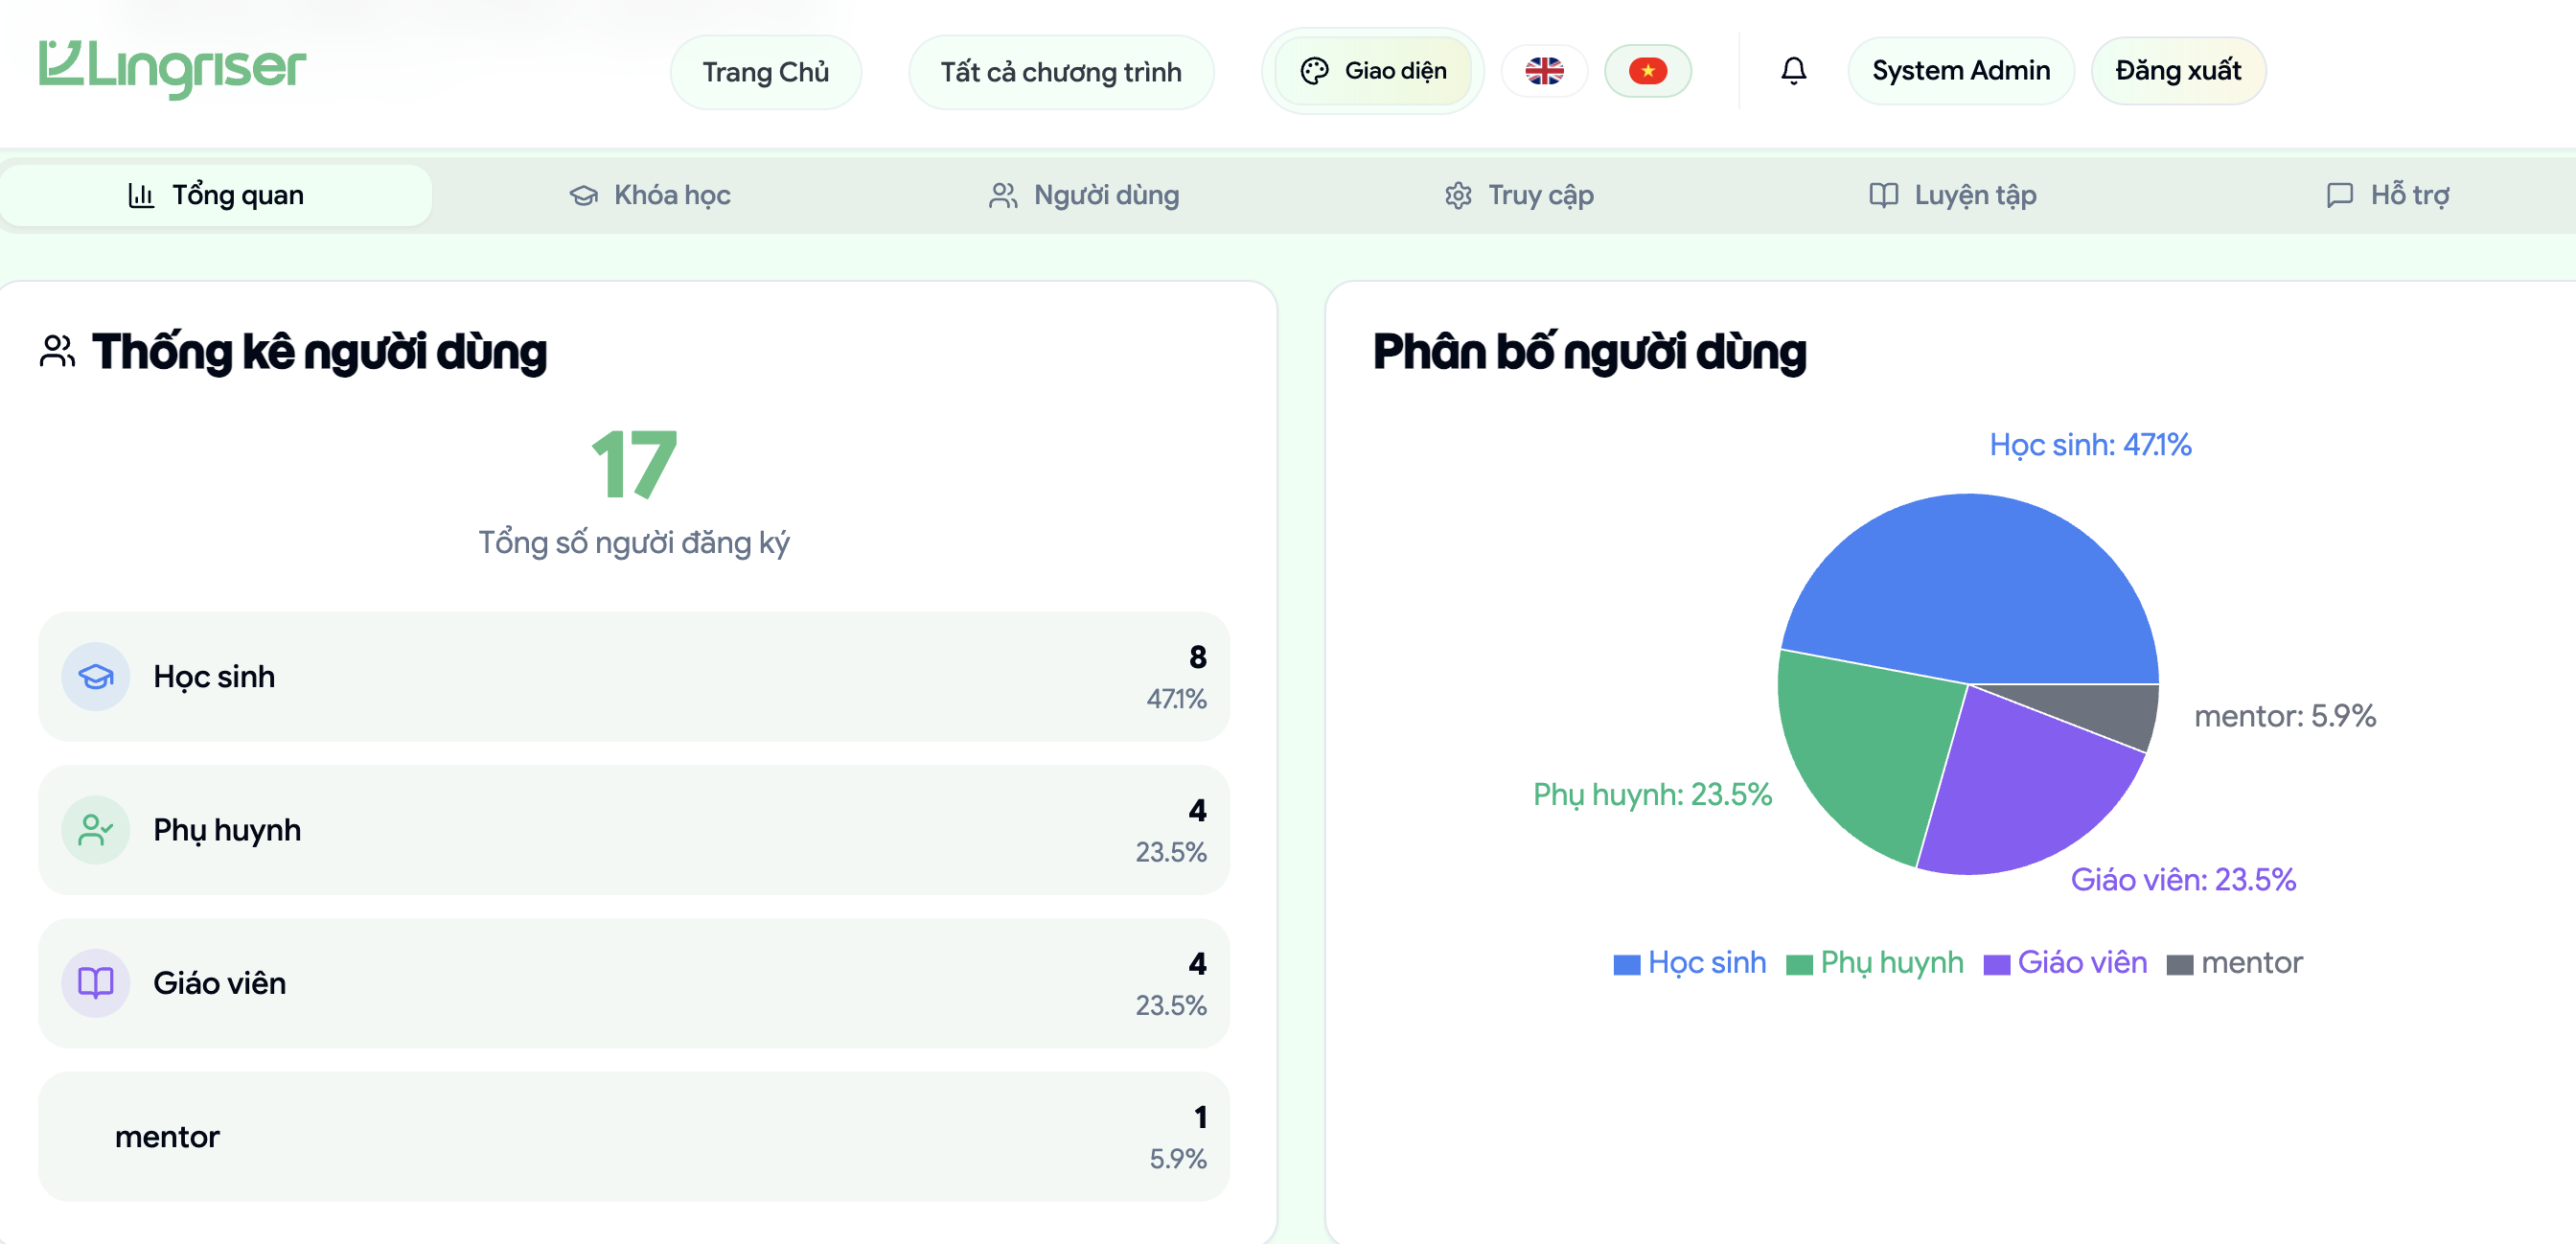
\includegraphics[width=\linewidth]{graphics/lingriser/admin.png}
    \captionsetup{skip=5pt}
    \caption{Bảng điều khiển quản trị của LingriserSpeaking}
    \label{fig:lingriser-admin-dashboard}
\end{figure}
\noindent Bảng điều khiển quản trị là khu vực vận hành toàn bộ hệ sinh thái LingriserSpeaking ở cấp độ hệ thống. Bố cục của màn hình nhấn mạnh các khối thống kê tổng quan kết hợp với các khu vực chuyên trách như quản lý người dùng, quản lý khóa học, theo dõi lượt truy cập, thống kê số phiên luyện tập và hỗ trợ hội thoại với người dùng. Cách tổ chức này cho phép quản trị viên vừa có cái nhìn khái quát về trạng thái nền tảng, vừa nhanh chóng đi sâu vào từng nhóm tác vụ vận hành cụ thể. Trong bối cảnh một nền tảng học tập có nhiều vai trò tương tác như LingriserSpeaking, giao diện admin đóng vai trò quan trọng trong việc duy trì tính ổn định, khả năng kiểm soát dữ liệu và chất lượng dịch vụ.


\section{Kết luận chương}
Chương này đã trình bày hệ thống wireframe cho các màn hình cốt lõi của nền tảng luyện thi tích hợp AI, từ các giao diện hướng đến người học cho đến các công cụ quản trị nội dung. Thông qua việc mô tả mục tiêu, bố cục và luồng tương tác của từng màn hình, chương đã làm rõ cách hệ thống hỗ trợ người dùng trong toàn bộ hành trình học tập: từ tiếp cận nền tảng, đăng nhập, lựa chọn bài luyện, làm bài, nhận phản hồi, tích lũy kiến thức đến theo dõi tiến độ cá nhân. Đây là cơ sở quan trọng để triển khai giao diện chi tiết, kiểm thử trải nghiệm người dùng và hiện thực hóa hệ thống trong các giai đoạn tiếp theo.